% Author: Wilker Aziz
% Contact: wilker.aziz@gmail.com 
% Documentation: http://en.wikibooks.org/wiki/LaTeX
% Equation editor: http://www.codecogs.com/latex/eqneditor.php

\documentclass[xcolor=pdftex,dvipsnames,table]{beamer}
\usefonttheme[onlymath]{serif}
%\usepackage{bm}
%\usepackage{beamerthemeshadow}
\setbeamertemplate{footline}[frame number]

%\usepackage{soul}
\usepackage{lmodern}
%\usetheme{Warsaw}
%\usetheme{Dresden}
%\usetheme{Amsterdam}

% allow the use of utf8 encoding
\usepackage{comment}
\usepackage{natbib}
\usepackage{graphicx}
\usepackage[absolute,overlay]{textpos}
\usepackage{pgf}
\usepackage{tikz}
\usepackage{tikz-qtree}
\usetikzlibrary{arrows,automata}
\usepackage{pbox}
\usepackage{amssymb}
\usepackage{ragged2e}
\usepackage{pifont}

\usepackage{commands}



% declares a document
\begin{document}


	\title{Decoding for SMT}
	\author{Wilker Aziz} 
	\institute[UvA]{
		%\inst{1}
		Universiteit van Amsterdam\\
		\texttt{w.aziz@uva.nl}
	}

	\date{\today}
	
	{
		\setbeamertemplate{footline}{}
		\frame{\titlepage}
	}

	% Table of contents	
	%\frame[allowframebreaks]
	\frame{
		\frametitle{Table of Contents}
		% commands the rendering of a table of contents
		\tableofcontents
	}

	% trick to start counting from the table of contents
	\setcounter{framenumber}{0}
	% trick to show the frame number and the total of frames at the bottom right corner
	\expandafter\def\expandafter\insertshorttitle\expandafter{%
		\insertshorttitle\hfill%
		\insertframenumber\,/\,\inserttotalframenumber
	}	
	
	\frame{
	\frametitle{Decoding for SMT}
	
	\pause 
	We will be reasoning \\ \pause
	\begin{center}
		making decisions
	\end{center}
	
	\pause
	
	~ about solutions \\ \pause
	\begin{center}
		structures (translations)
	\end{center}
	
	\pause
	
	~ under a statistical model \\ \pause
	\begin{center}
		a function / a partial ordering
	\end{center}
	
	
}

\frame{
	\frametitle{Keywords}
	
	We need to better characterise 
	
	\begin{enumerate}
		\item<2-> space of solutions \\
		\textcolor{blue}{get to know the terrain}
		\item<3-> statistical model \\
		\textcolor{blue}{how to assess the importance of things}
		\item<4-> decision rules \\
		\textcolor{blue}{know what you want}
	\end{enumerate}
	
	
}

\frame{
	\frametitle{Terrain}
	
	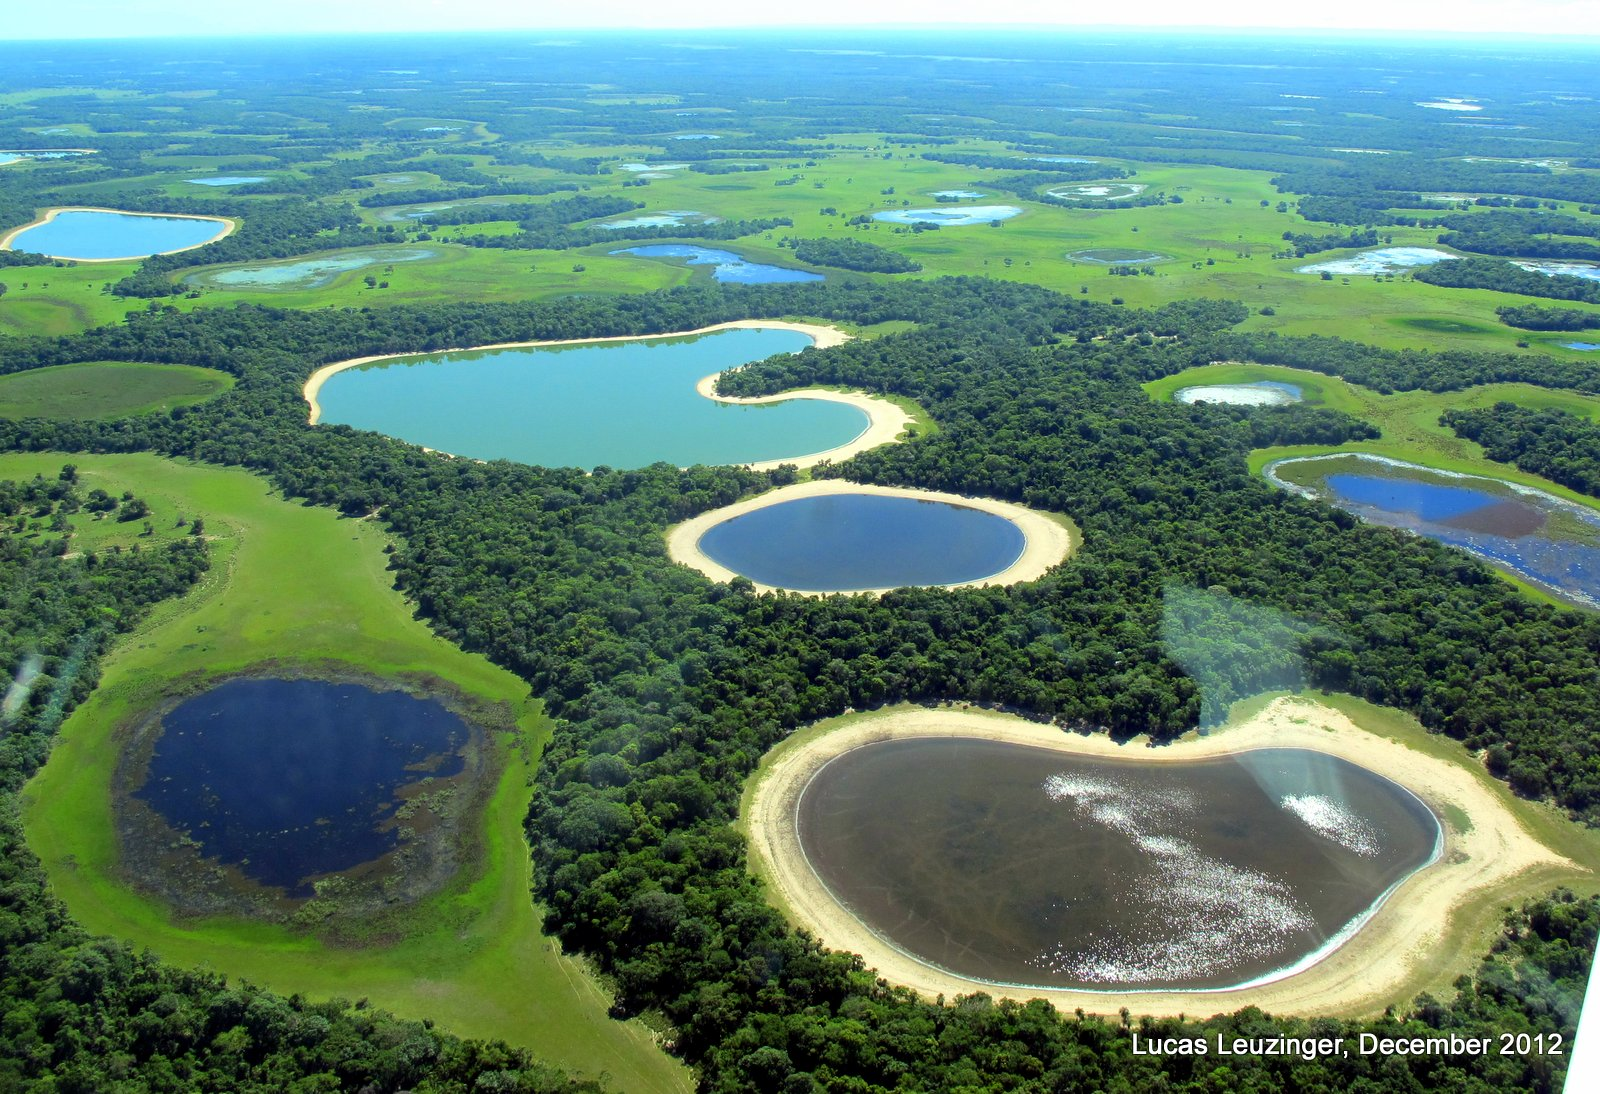
\includegraphics[scale=0.4]{img/pantanal} \pause
	
	not everywhere is a good place to stand
}

\frame{
	\frametitle{The importance (or cost) of things}
	
		
		\only<1>{
	
		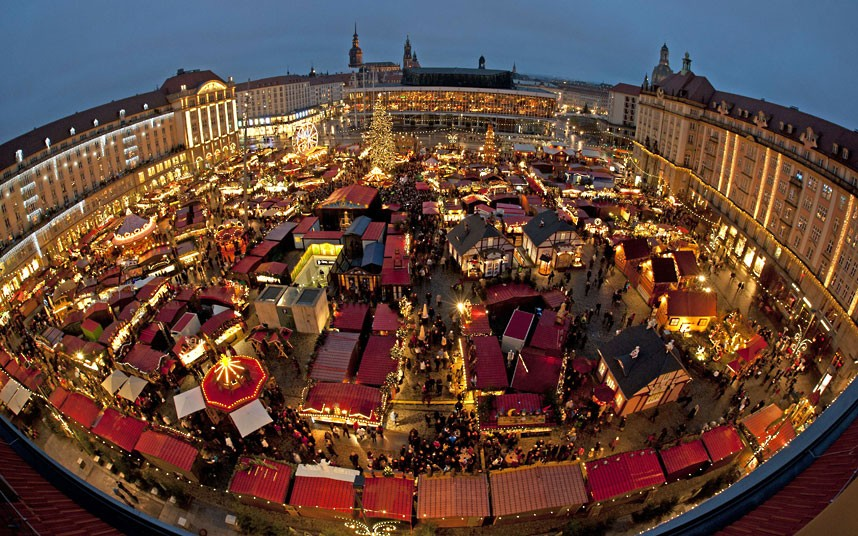
\includegraphics[scale=0.3]{img/demarket} 
		
		German xmas market
		
		}

		\only<2>{
		
		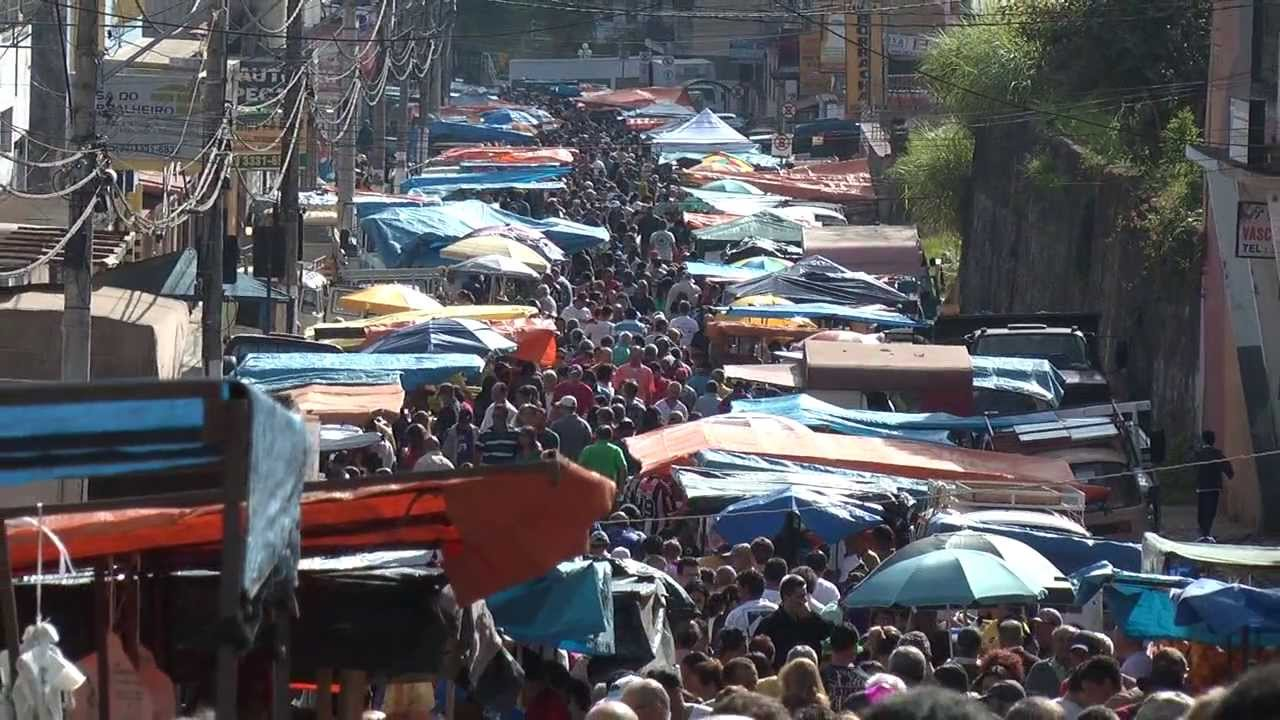
\includegraphics[scale=0.2]{img/brmarket}
		
		Brazilian street market
		
		}
		\only<3-6>{
		
			German xmas market
			\begin{columns}
				\begin{column}{0.4\textwidth}
					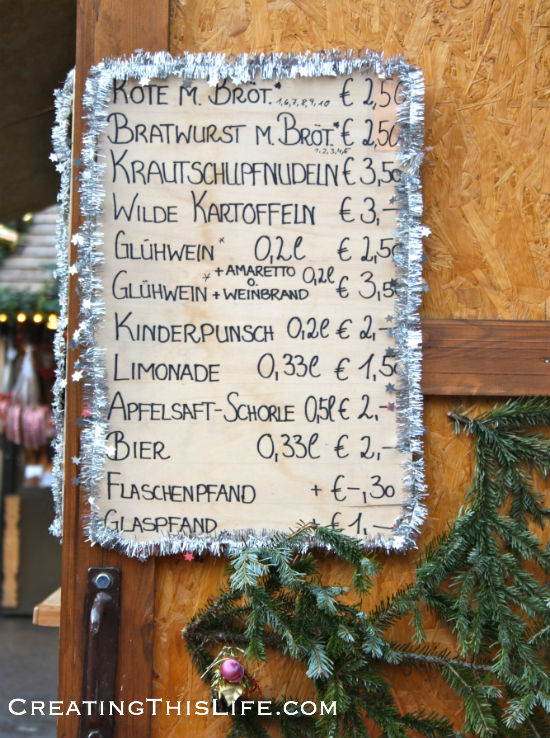
\includegraphics[scale=0.2]{img/demenu}
				\end{column}
				\begin{column}{0.45\textwidth}
					Price of product depends on
					\begin{itemize}
						\item<4-> the product
						\item<5-> brand
						\item<6-> quality of service
					\end{itemize}
				\end{column}
			\end{columns}
		}

		\only<7->{
		
			Brazilian street market
			\begin{columns}
				\begin{column}{0.4\textwidth}
					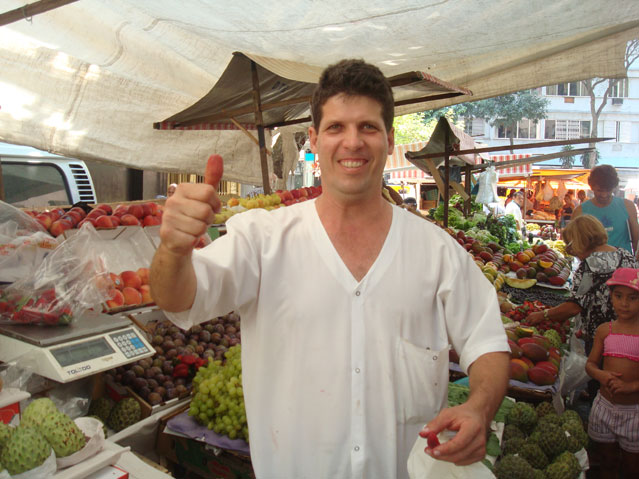
\includegraphics[scale=0.2]{img/feirante}
				\end{column}
				\begin{column}{0.45\textwidth}
					Price of product depends on
					\begin{itemize}
						\item the product
						\item brand
						\item quality of service
						\item<8-> seller's mood
						\item<9-> your look
						\item<10-> products you acquired from other stalls
						\item<11-> from whom you bought those
					\end{itemize}
				\end{column}
			\end{columns}
		}

}

\frame{
	\frametitle{Know what you want}
	
	\only<1>{
		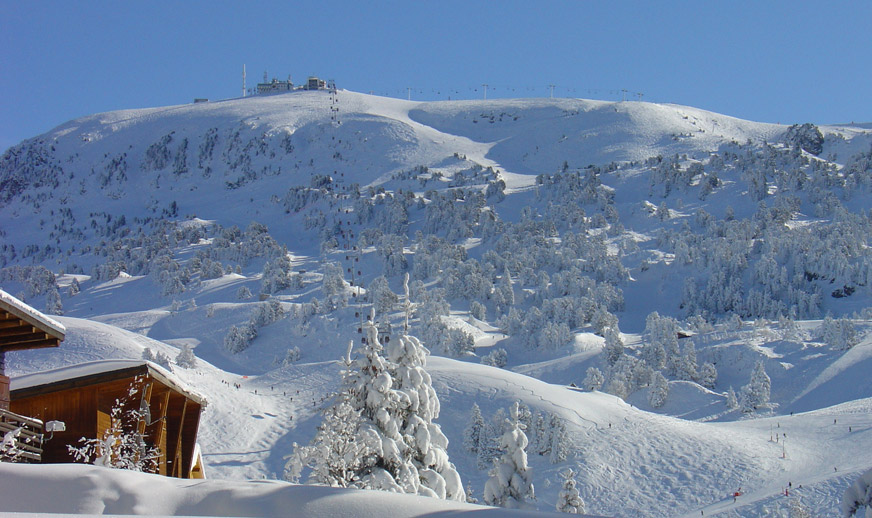
\includegraphics[scale=0.3]{img/station}
		
		what do you think when you see this picture?
	}
	\only<2>{
		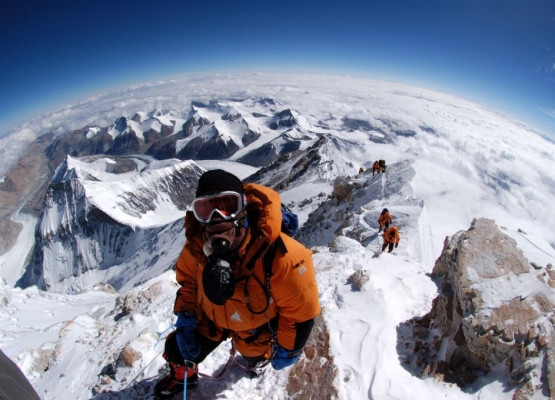
\includegraphics[scale=0.4]{img/top}
		
		make a selfie (and lose a couple of fingers in the process)?
	}
	\only<3>{
		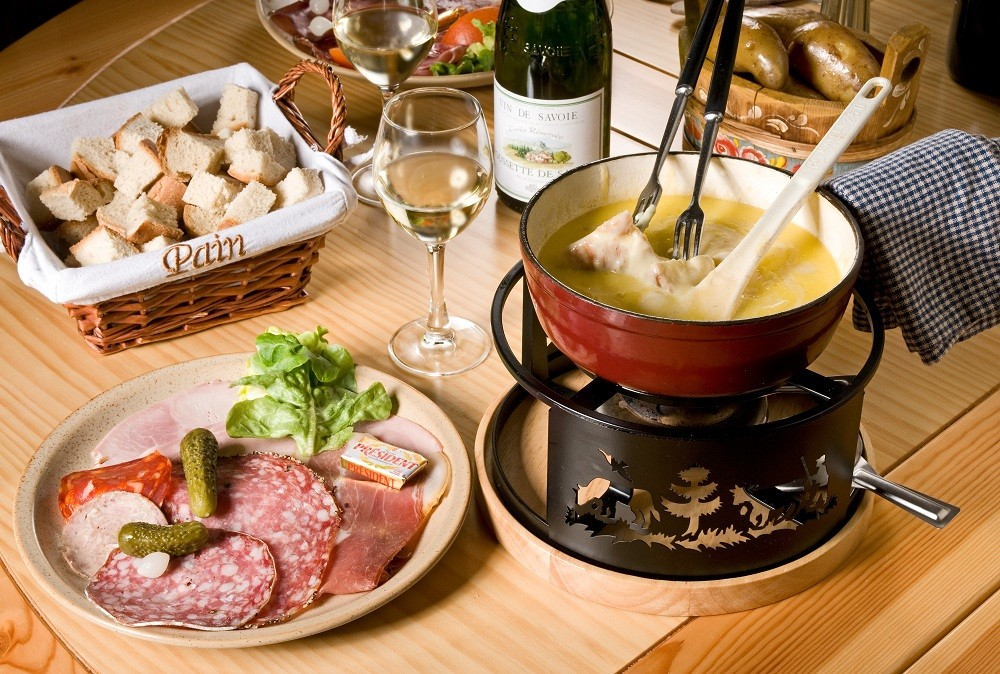
\includegraphics[scale=0.25]{img/dinner}
		
		French goodies in a cozy chalet?
	}
}


	\section{Monotone word replacement models}

\frame{
	\frametitle{Model of translational equivalences}

	Defines the space of possible translations \\
	\begin{itemize}
		\item think of it as a recipe to generate translations
	\end{itemize}
	
	\pause
	\pause
	Example:	\\

	\begin{itemize}
		\item a word replacement model \\ \pause
		\item operates in monotone left-to-right order \pause
		\item with no insertions or deletions \pause
		\item constrained to known word-to-word bilingual mappings \\
		(rule set)
	\end{itemize}
}


\frame{
	\frametitle{Monotone word-by-word translation: solutions}
	\only<1>{
Source: \ftext{um conto de duas cidades}\\

Translation rules\footnote{Unrealistically simple} \\
\begin{tabular}{l l}
\ftext{um} & \{\etext{a}, \etext{some}, \etext{one}\} \\
\ftext{conto} & \{\etext{tale}, \etext{story}, \etext{narrative}, \etext{novella}\} \\
\ftext{de} & \{\etext{of}, \etext{from}, \etext{'s}\} \\
\ftext{duas} & \{\etext{two}, \etext{couple}\} \\
\ftext{cidades} & \{\etext{cities}, \etext{towns}, \etext{villages}\} \\
\end{tabular}
}
\only<2->{
\begin{textblock*}{63mm}(0.6\textwidth,0.15\textheight)
\begin{footnotesize}
\begin{tabular}{l l}
\ftext{um} & \{\etext{a}, \etext{some}, \etext{one}\} \\
\ftext{conto} & \{\etext{tale}, \etext{story}, \etext{narrative}, \etext{novella}\} \\
\ftext{de} & \{\etext{of}, \etext{from}, \etext{'s}\} \\
\ftext{duas} & \{\etext{two}, \etext{couple}\} \\
\ftext{cidades} & \{\etext{cities}, \etext{towns}, \etext{villages}\} \\
\end{tabular}
\end{footnotesize}
\end{textblock*}

\ftext{um conto de duas cidades}\\
}
\only<3->{
\etext{a tale of two cities}\\
}
\only<4->{
\etext{a tale of two \bf towns}\\
}
\only<5->{
\etext{a tale of two \bf villages}\\
}
\only<6->{
\etext{a tale of \bf couple cities}\\
}
\only<7->{
\etext{a tale of couple \bf towns}\\
}
%\only<8->{
%\etext{a tale of couple \bf villages}\\
%}
%\only<9->{
%\etext{a tale \bf from two cities}\\
%}
%\only<10->{
%\etext{a tale from two \bf towns}\\
%}
%\only<11->{
%\etext{a tale from two \bf villages}\\
%}
%\only<12->{
%\etext{a tale from \bf couple cities}\\
%}
%\only<13->{
%\etext{a tale from couple \bf towns}\\
%}
%\only<14->{
%\etext{a tale from couple \bf villages}\\
%}
\only<8->{
\etext{...}\\

\begin{textblock*}{63mm}(0.6\textwidth,0.75\textheight)
This can go very far :(
\end{textblock*}
}

}


\frame{
	\frametitle{Monotone word-by-word translation: complexity}
	
	Say
	\begin{itemize}
		\item the input has $I$ words \\
		\item we know at most $t$ translation options per source word
	\end{itemize}
	
	\pause
	This makes $O(t^I)$ solutions\\
	
	\pause
	Note
	\begin{itemize}
		\item WMT14's shared task: $I=40$ on average
		\item last I checked Moses default was $t = 100$ \\
		\hfill (for a more complex model)
		\item silly monotone word replacement model: $10^{80}$ solutions
	\end{itemize}
	
}


\frame{
	\frametitle{Representing discrete sets efficiently}
	\begin{textblock*}{63mm}(0.6\textwidth,0.15\textheight)

\begin{footnotesize}
\begin{tabular}{l l}
\ftext{um} & \{\etext{a}, \etext{some}, \etext{one}\} \\
\ftext{conto} & \{\etext{tale}, \etext{story}, \etext{narrative}, \etext{novella}\} \\
\ftext{de} & \{\etext{of}, \etext{from}, \etext{'s}\} \\
\ftext{duas} & \{\etext{two}, \etext{couple}\} \\
\ftext{cidades} & \{\etext{cities}, \etext{towns}, \etext{villages}\} \\
\end{tabular}
\end{footnotesize}

\end{textblock*}

\begin{textblock*}{63mm}(0.1\textwidth,0.50\textheight)
\scalebox{0.6}{

\begin{tikzpicture}[->,>=stealth',shorten >=1pt,auto,node distance=2.8cm,semithick]
  	\tikzstyle{every state}=[draw=black,text=black]

\node[initial,state,style={initial text=}] (A) {$0$};
\node[state] (B) [right of=A] {$1$};
\node[state] (C) [right of=B] {$2$};
\node[state] (D) [right of=C] {$3$};
\node[state] (E) [right of=D] {$4$};
\node[state,accepting] [right of=E] (F) {$5$};

\only<1>{\path[color=red] (A) edge node {\ftext{um}} (B);}
\only<1-2>{\path[color=red] (B) edge node {\ftext{conto}} (C);}
\only<1-3>{\path[color=red] (C) edge node {\ftext{de}} (D);}
\only<1-4>{\path[color=red] (D) edge node {\ftext{duas}} (E);}
\only<1-5>{\path[color=red] (E) edge node {\ftext{cidades}} (F);}
	
\only<2->{
	\path[color=blue] 
		(A) edge node {\etext{a}} (B)
			edge [bend right] node {\etext{some}} (B)
			edge [bend left] node {\etext{one}} (B);
}
\only<3->{
	\path[color=blue] 
		(B) edge node {\etext{narrative}} (C)
			edge [bend right] node {\etext{tale}} (C)
			edge [bend left] node {\etext{story}} (C)
			edge [bend right=60] node [below] {novella} (C);
}
\only<4->{
	\path[color=blue] 
		(C) edge node {\etext{of}} (D)
			edge [bend right] node {\etext{from}} (D)
			edge [bend left] node {\etext{'s}} (D);
}
\only<5->{
	\path[color=blue] 
		(D) edge [bend left] node {\etext{two}} (E)
			edge [bend right] node {\etext{couple}} (E);
}
\only<6->{
	\path[color=blue] 
		(E) edge node {\etext{cities}} (F)
			edge [bend right] node {\etext{towns}} (F)
			edge [bend left] node {\etext{villages}} (F);
}			
\end{tikzpicture} 

}
\end{textblock*}


\only<7>{
	\begin{textblock*}{63mm}(0.2\textwidth,0.7\textheight)
	$3 \times 4 \times 3 \times 2 \times 3 = 216$ solutions
	\begin{itemize}
		\item $6$ states
		\item $3 + 4 + 3 + 2 + 3 = 15$ transitions
	\end{itemize}
	\end{textblock*}
}

}

\frame{
	\frametitle{Packing solutions with finite-state automata}
	Same $O(t^I)$ solutions using
	\begin{itemize}
		\item $O(I)$ states
		\item $O(tI)$ transitions
	\end{itemize}
}

\frame{
	\frametitle{Monotone word-by-word translation: expressiveness}
	
	
	Given the ``recipe'' and the set of known mappings \pause
	\begin{enumerate}	
		\item what sentences can we translate? \pause
		\item what translations do we produce? \pause
	\end{enumerate}


	What is the set of sentence pairs defined by this model?
}


\frame{
	\frametitle{Monotone word-by-word translation: expressiveness}

	\only<1>{
Consider this extended set of rules\footnote{Unrealistically simple}\\
\begin{tabular}{l l}
\ftext{um} & \{\etext{a}, \etext{some}, \etext{one}\} \\
\ftext{conto} & \{\etext{tale}, \etext{story}, \etext{narrative}, \etext{novella}\} \\
\ftext{de} & \{\etext{of}, \etext{from}, \etext{'s}\} \\
\ftext{duas} & \{\etext{two}, \etext{couple}\} \\
\ftext{cidades} & \{\etext{cities}, \etext{towns}, \etext{villages}\} \\
\ftext{nosso} & \{\etext{our}, \etext{ours}\} \\
\ftext{amigo} & \{\etext{friend}, \etext{mate}\} \\
\ftext{comum} & \{\etext{ordinary}, \etext{common}, \etext{usual}, \etext{mutual}\} \\

\end{tabular}
}
\only<2->{
\begin{textblock*}{63mm}(0.6\textwidth,0.15\textheight)
\begin{scriptsize}
\begin{tabular}{l l}
\ftext{um} & \{\etext{a}, \etext{some}, \etext{one}\} \\
\ftext{conto} & \{\etext{tale}, \etext{story}, \etext{narrative}, \etext{novella}\} \\
\ftext{de} & \{\etext{of}, \etext{from}, \etext{'s}\} \\
\ftext{duas} & \{\etext{two}, \etext{couple}\} \\
\ftext{cidades} & \{\etext{cities}, \etext{towns}, \etext{villages}\} \\
\ftext{nosso} & \{\etext{our}, \etext{ours}\} \\
\ftext{amigo} & \{\etext{friend}, \etext{mate}\} \\
\ftext{comum} & \{\etext{ordinary}, \etext{common}, \etext{usual}, \etext{mutual}\} \\

\end{tabular}
\end{scriptsize}
\end{textblock*}
}


\begin{textblock*}{63mm}(0.6\textwidth,0.6\textheight)
\only<3->{some of the source sentences...\\}
\only<8->{some of the target sentences...\\}

\only<17->{\vspace{5pt}{\color{OliveGreen}an {\bf infinite} set of source sentences}}
\only<18->{{\color{OliveGreen}each of which has an exponential number of translations}}
\end{textblock*}


\only<3->{\ftext{um conto de duas cidades}\\}
\only<8->{~\etext{a tale of two cities}\\}
\only<9->{~\etext{a tale of two \bf towns}\\}
\only<10->{~\etext{a tale of two \bf villages}\\~\etext{...}\\}
\only<4->{\ftext{{\bf nosso} conto de duas cidades}\\}
\only<11->{~\etext{our story 's couple towns}\\}
\only<12->{~\etext{{\bf ours} story 's couple towns}\\~\etext{...}\\}
\only<5->{\ftext{nosso {\bf amigo} de duas cidades}\\}
\only<13->{~\etext{...}\\}
\only<6->{\ftext{nosso amigo {\bf comum}}\\}
\only<14->{~\etext{...}\\}
\only<7->{\ftext{{\bf um} amigo comum}\\}
\only<15->{~\etext{...}\\}
\only<16->{\ftext{um conto de duas cidades de um amigo comum nosso ...}\\\ftext{...}\\}

%	\begin{textblock*}{63mm}(0.6\textwidth,0.75\textheight)
%	This can go very far...
%	\end{textblock*}

%	\begin{textblock*}{63mm}(0.6\textwidth,0.8\textheight)
%	and it does go {\bf very} far!
%	\end{textblock*}	
}

\frame{
	\frametitle{Compact representation}

	\only<1-2>{Call $R$ the set of rules \\}
\only<2>{
	\begin{center}
	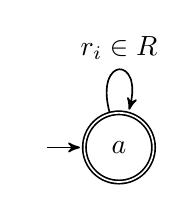
\begin{tikzpicture}[->,>=stealth',shorten >=1pt,auto,node distance=2.8cm,semithick]
	  	\tikzstyle{every state}=[draw=black,text=black]

  		\node[initial,accepting,state,style={initial text=}] (A)                    {$a$};
	
		\path (A) edge [loop above] node {$r_i \in R$} (A);

	\end{tikzpicture}
	\end{center}
}
\only<3>{
	Example \\
	\begin{center}
	\scalebox{0.8}{
	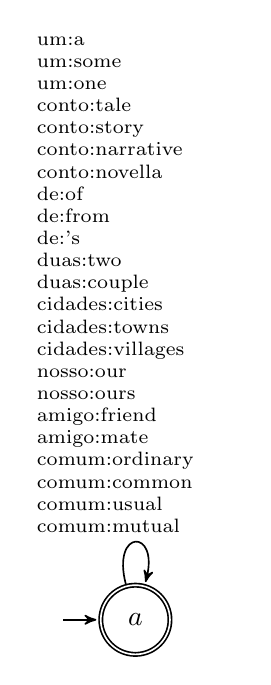
\begin{tikzpicture}[->,>=stealth',shorten >=1pt,auto,node distance=2.8cm,semithick]
	  	\tikzstyle{every state}=[draw=black,text=black]

  		\node[initial,accepting,state,style={initial text=}] (A)                    {$a$};
	
		\path (A) edge [loop above] node {%
			\pbox{4cm}{\scriptsize
				\ftext{um}:\etext{a} \\
				\ftext{um}:\etext{some} \\
				\ftext{um}:\etext{one} \\
				\ftext{conto}:\etext{tale} \\
				\ftext{conto}:\etext{story} \\
				\ftext{conto}:\etext{narrative} \\
				\ftext{conto}:\etext{novella} \\
				\ftext{de}:\etext{of} \\
				\ftext{de}:\etext{from} \\
				\ftext{de}:\etext{'s} \\
				\ftext{duas}:\etext{two} \\
				\ftext{duas}:\etext{couple} \\
				\ftext{cidades}:\etext{cities} \\
				\ftext{cidades}:\etext{towns} \\
				\ftext{cidades}:\etext{villages} \\
				\ftext{nosso}:\etext{our} \\
				\ftext{nosso}:\etext{ours} \\
				\ftext{amigo}:\etext{friend} \\
				\ftext{amigo}:\etext{mate} \\
				\ftext{comum}:\etext{ordinary} \\
				\ftext{comum}:\etext{common} \\
				\ftext{comum}:\etext{usual} \\
				\ftext{comum}:\etext{mutual}
			}						
		} (A);

	\end{tikzpicture}}
	\end{center}
}

}


\frame{
	\frametitle{Space of solutions as intersection}
	
	\begin{center}
	``From the set of sentence pairs compatible with the model, \\
	retain those matching this input''
	\end{center}
	
}

\frame{
	\frametitle{Space of solutions as intersection/composition}
	
	%
% TRANSLATION RULES
%
\begin{textblock*}{63mm}(0.99\textwidth,0.1\textheight)
\scalebox{0.75}{

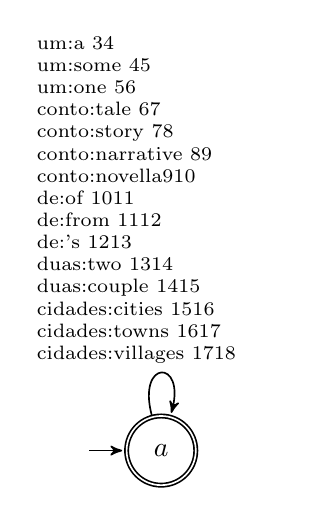
\begin{tikzpicture}[->,>=stealth',shorten >=1pt,auto,node distance=2.8cm,semithick]
  	\tikzstyle{every state}=[draw=black,text=black]

  		\node[initial,accepting,state,style={initial text=}] (A)                    {$a$};

	\path (A) edge [loop above] node {%
		\pbox{4cm}{\scriptsize
			\ftext{um}:\etext{a} \lefttik{3}{4} \\
			\ftext{um}:\etext{some} \lefttik{4}{5} \\
			\ftext{um}:\etext{one} \lefttik{5}{6} \\
			\ftext{conto}:\etext{tale} \lefttik{6}{7} \\
			\ftext{conto}:\etext{story} \lefttik{7}{8}\\
			\ftext{conto}:\etext{narrative} \lefttik{8}{9}\\
			\ftext{conto}:\etext{novella}\lefttik{9}{10}\\
			\ftext{de}:\etext{of} \lefttik{10}{11}\\
			\ftext{de}:\etext{from} \lefttik{11}{12}\\
			\ftext{de}:\etext{'s} \lefttik{12}{13}\\
			\ftext{duas}:\etext{two} \lefttik{13}{14}\\
			\ftext{duas}:\etext{couple} \lefttik{14}{15}\\
			\ftext{cidades}:\etext{cities} \lefttik{15}{16}\\
			\ftext{cidades}:\etext{towns} \lefttik{16}{17}\\
			\ftext{cidades}:\etext{villages} \lefttik{17}{18}
		}						
	} (A);

\end{tikzpicture}
} % scale-box
\end{textblock*}

%
% INPUT
%
\begin{textblock*}{63mm}(0.01\textwidth,0.2\textheight)
\scalebox{0.6}{	
\begin{tikzpicture}[->,>=stealth',shorten >=1pt,auto,node distance=2.8cm,semithick]
  	\tikzstyle{every state}=[draw=black,text=black]
  	\node[initial,state,style={initial text=}] (A) {$0$};
\node[state] (B) [right of=A] {$1$};
\node[state] (C) [right of=B] {$2$};
\node[state] (D) [right of=C] {$3$};
\node[state] (E) [right of=D] {$4$};
\node[state,accepting] [right of=E] (F) {$5$};
\path[color=red] 
	(A) edge node {\ftext{um}\only<3-5>{$^\star$}} (B)
	(B) edge node {\ftext{conto}\only<6-9>{$^\star$}} (C)
	(C) edge node {\ftext{de}\only<10-12>{$^\star$}} (D)
	(D) edge node {\ftext{duas}\only<13-14>{$^\star$}} (E)
	(E) edge node {\ftext{cidades}\only<15-17>{$^\star$}} (F);
\end{tikzpicture} 
}
\end{textblock*}

%
% INTERSECTION
%
\begin{textblock*}{63mm}(0.01\textwidth,0.45\textheight)
\scalebox{0.65}{

\begin{tikzpicture}[->,>=stealth',shorten >=1pt,auto,node distance=2.8cm,semithick]
  	\tikzstyle{every state}=[draw=black,text=black]
\tikzstyle{every path}=[draw=blue,text=blue]

\only<2->{
\node[initial,state,style={initial text=}] (A) {$0,a$};
\node[state] (B) [right of=A] {$1,a$};
\node[state] (C) [right of=B] {$2,a$};
\node[state] (D) [right of=C] {$3,a$};
\node[state] (E) [right of=D] {$4,a$};
\node[state,accepting] [right of=E] (F) {$5,a$};
}

	
\only<3->{\path (A) edge [bend left] node {\etext{a}} (B);}
\only<4->{\path (A) edge node {\etext{some}} (B);}
\only<5->{\path (A) edge [bend right] node {\etext{one}} (B);}

\only<6->{\path (B) edge [bend left] node {\etext{tale}} (C);}
\only<7->{\path (B) edge node {\etext{story}} (C);}
\only<8->{\path (B) edge [bend right] node {\etext{narrative}} (C);}
\only<9->{\path (B) edge [bend right=60] node [below] {novella} (C);}

\only<10->{\path (C) edge [bend left] node {\etext{of}} (D);}
\only<11->{\path (C) edge node {\etext{from}} (D);}
\only<12->{\path (C) edge [bend right] node {\etext{'s}} (D);}

\only<13->{\path (D) edge [bend left] node {\etext{two}} (E);}
\only<14->{\path (D) edge [bend right] node {\etext{couple}} (E);}

\only<15->{\path(E) edge [bend left] node {\etext{cities}} (F);}
\only<16->{\path(E) edge node {\etext{towns}} (F);}
\only<17->{\path(E) edge [bend right] node {\etext{villages}} (F);}			
\end{tikzpicture} 

}
\end{textblock*}	

}

\frame{
	\frametitle{Recap 1}
	
	\pause
	Model of translational equivalences 
	\begin{itemize}
		\item defines the space of possible sentence pairs
		\item conveniently decomposes into smaller bilingual mappings
	\end{itemize}
	\pause
	Monotone word replacement model
	\begin{itemize}
		\item easy to represent using finite-state transducers \pause
		\item set of translations given by intersection \pause
		\item exponential number of solutions in linear space \pause
		\item translates infinitely many sentences \\
		\pause {\bf {\color{red}but not nearly enough interesting cases!}}
	\end{itemize}
}


\frame{
	\frametitle{Monotone word-by-word translation: fail!}
	
		
\begin{textblock*}{63mm}(0.1\textwidth,0.25\textheight)
\begin{small}
\begin{tabular}{l l}
\ftext{nosso} & \{\etext{our}, \etext{ours}\} \\
\ftext{amigo} & \{\etext{friend}, \etext{mate}\}\\
\ftext{comum} & \{\etext{ordinary}, \etext{common}, \etext{usual}, \etext{mutual}\} \\
\end{tabular}
\end{small}
\end{textblock*}

\begin{textblock*}{90mm}(0.1\textwidth,0.50\textheight)
\scalebox{0.7}{

\begin{tikzpicture}[->,>=stealth',shorten >=1pt,auto,node distance=2.8cm,semithick]
  	\tikzstyle{every state}=[draw=black,text=black]

\node[initial,state,style={initial text=}] (A) {$0$};
\node[state] (B) [right of=A] {$1$};
\node[state] (C) [right of=B] {$2$};
\node[state,accepting] (D) [right of=C] {$3$};

\only<1>{\path[color=red] (A) edge node {\ftext{nosso}} (B);}
\only<1-2>{\path[color=red] (B) edge node {\ftext{amigo}} (C);}
\only<1-3>{\path[color=red] (C) edge node {\ftext{comum}} (D);}
	
\only<2->{
	\path[color=blue] 
		(A) edge [bend right] node {\etext{our}} (B)
			edge [bend left] node {\etext{ours}} (B);
}
\only<3->{
	\path[color=blue] 
		(B) edge [bend right] node {\etext{mate}} (C)
			edge [bend left] node {\etext{friend}} (C);
}
\only<4->{
	\path[color=blue] 
		(C) edge node {\etext{common}} (D)
			edge [bend right] node {\etext{usual}} (D)
			edge [bend left] node {\etext{ordinary}} (D)
			edge [bend right=60] node [below] {mutual} (D);
}
\end{tikzpicture} 
}


\only<5->{
	\vspace{5pt}
	We simply cannot obtain a correct translation \\
	\begin{center}\color{OliveGreen}
	our mutual friend
	\end{center}
}

\end{textblock*}
}

	\section{Reordering}

\subsection{Unconstrained}

\frame{
	\frametitle{Reordering}
	
	\only<1>{
	Our model of translational equivalences assumes monotonicity 
	\begin{itemize}
		\item a word replacement model 	
		\item {\color{red}operates in {\bf monotone} left-to-right order}		
		\item with no insertions or deletions
		\item constrained to known word-to-word bilingual mappings \\
	(rule set)
	\end{itemize}
	}
	\only<2->{
	Not anymore!
	\begin{itemize}
		\item a word replacement model	
		\item {\color{blue}operates in {\bf arbitrary} order}
		\item with no insertions or deletions
		\item constrained to known word-to-word bilingual mappings \\
	(rule set)
	\end{itemize}
	}
}

\frame{
	\frametitle{Translating arbitrary permutations}
		
\begin{columns}
\begin{column}{0.5\linewidth}
\only<1->{\ftext{nosso amigo comum} \\}
\only<1->{
\scalebox{0.5}{
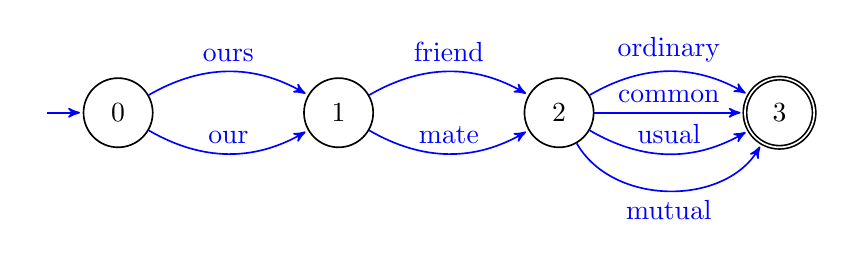
\begin{tikzpicture}[->,>=stealth',shorten >=1pt,auto,node distance=2.8cm,semithick]
\tikzstyle{every state}=[draw=black,text=black]
\tikzstyle{every path}=[draw=blue,text=blue]	

\node[initial,state,style={initial text=}] (A) {$0$};
\node[state] (B) [right of=A] {$1$};
\node[state] (C) [right of=B] {$2$};
\node[state,accepting] (D) [right of=C] {$3$};
	\path
		(A) edge [bend right] node {\etext{our}} (B)
			edge [bend left] node {\etext{ours}} (B)
		(B) edge [bend right] node {\etext{mate}} (C)
			edge [bend left] node {\etext{friend}} (C)
		(C) edge node {\etext{common}} (D)
			edge [bend right] node {\etext{usual}} (D)
			edge [bend left] node {\etext{ordinary}} (D)
			edge [bend right=60] node [below] {mutual} (D);
\end{tikzpicture} 
}
}

\only<3->{\ftext{nosso comum amigo} \\}
\only<3->{
\scalebox{0.5}{
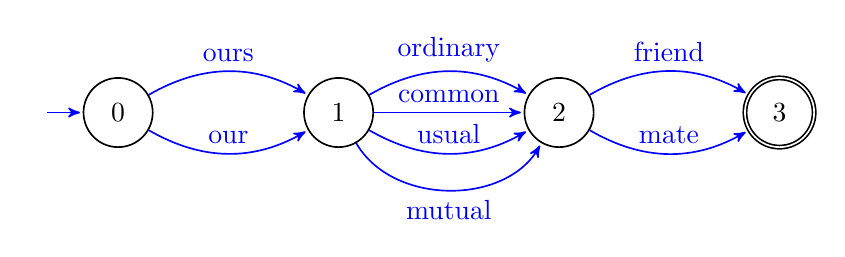
\begin{tikzpicture}[->,>=stealth',shorten >=1pt,auto,node distance=2.8cm,semithick]
\tikzstyle{every state}=[draw=black,text=black]
\tikzstyle{every path}=[draw=blue,text=blue]	

\node[initial,state,style={initial text=}] (A) {$0$};
\node[state] (B) [right of=A] {$1$};
\node[state] (C) [right of=B] {$2$};
\node[state,accepting] (D) [right of=C] {$3$};
	\path
		(A) edge [bend right] node {\etext{our}} (B)
			edge [bend left] node {\etext{ours}} (B)
		(B) edge node {\etext{common}} (C)
			edge [bend right] node {\etext{usual}} (C)
			edge [bend left] node {\etext{ordinary}} (C)
			edge [bend right=60] node [below] {mutual} (C)
		(C) edge [bend right] node {\etext{mate}} (D)
			edge [bend left] node {\etext{friend}} (D);
	
\end{tikzpicture} 
}
}

\only<5->{\ftext{amigo comum nosso} \\}
\only<5->{
\scalebox{0.5}{
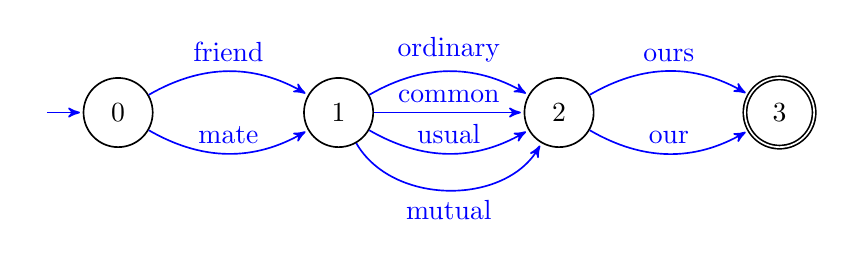
\begin{tikzpicture}[->,>=stealth',shorten >=1pt,auto,node distance=2.8cm,semithick]
\tikzstyle{every state}=[draw=black,text=black]
\tikzstyle{every path}=[draw=blue,text=blue]	

\node[initial,state,style={initial text=}] (A) {$0$};
\node[state] (B) [right of=A] {$1$};
\node[state] (C) [right of=B] {$2$};
\node[state,accepting] (D) [right of=C] {$3$};
	\path
		(A) edge [bend right] node {\etext{mate}} (B)
			edge [bend left] node {\etext{friend}} (B)
		(B) edge node {\etext{common}} (C)
			edge [bend right] node {\etext{usual}} (C)
			edge [bend left] node {\etext{ordinary}} (C)
			edge [bend right=60] node [below] {mutual} (C)
		(C) edge [bend right] node {\etext{our}} (D)
			edge [bend left] node {\etext{ours}} (D);
\end{tikzpicture} 
}
}
\end{column}
\begin{column}{0.5\linewidth}
\only<2->{\ftext{amigo nosso comum} \\}
\only<2->{
\scalebox{0.5}{
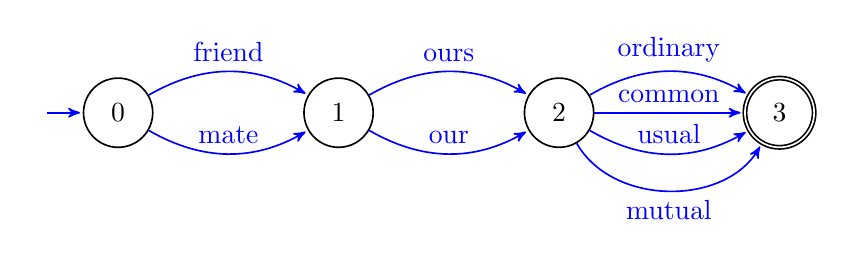
\begin{tikzpicture}[->,>=stealth',shorten >=1pt,auto,node distance=2.8cm,semithick]
\tikzstyle{every state}=[draw=black,text=black]
\tikzstyle{every path}=[draw=blue,text=blue]	

\node[initial,state,style={initial text=}] (A) {$0$};
\node[state] (B) [right of=A] {$1$};
\node[state] (C) [right of=B] {$2$};
\node[state,accepting] (D) [right of=C] {$3$};
	\path
		(A) edge [bend right] node {\etext{mate}} (B)
			edge [bend left] node {\etext{friend}} (B)
		(B) edge [bend right] node {\etext{our}} (C)
			edge [bend left] node {\etext{ours}} (C)
		(C) edge node {\etext{common}} (D)
			edge [bend right] node {\etext{usual}} (D)
			edge [bend left] node {\etext{ordinary}} (D)
			edge [bend right=60] node [below] {mutual} (D);			
\end{tikzpicture} 
}
}
\only<4->{\ftext{comum nosso amigo} \\}
\only<4->{
\scalebox{0.5}{
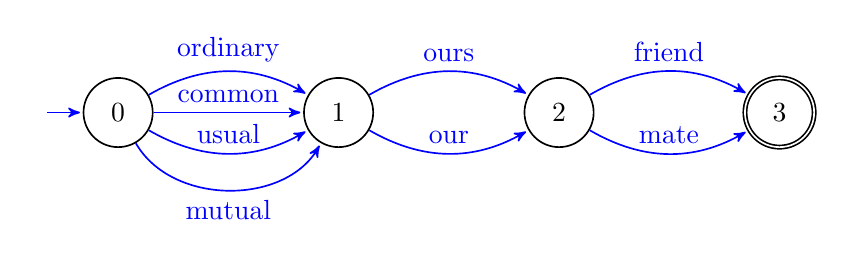
\begin{tikzpicture}[->,>=stealth',shorten >=1pt,auto,node distance=2.8cm,semithick]
\tikzstyle{every state}=[draw=black,text=black]
\tikzstyle{every path}=[draw=blue,text=blue]	

\node[initial,state,style={initial text=}] (A) {$0$};
\node[state] (B) [right of=A] {$1$};
\node[state] (C) [right of=B] {$2$};
\node[state,accepting] (D) [right of=C] {$3$};
	\path
		(A) edge node {\etext{common}} (B)
			edge [bend right] node {\etext{usual}} (B)
			edge [bend left] node {\etext{ordinary}} (B)
			edge [bend right=60] node [below] {mutual} (B)
		(B) edge [bend right] node {\etext{our}} (C)
			edge [bend left] node {\etext{ours}} (C)				
		(C) edge [bend right] node {\etext{mate}} (D)
			edge [bend left] node {\etext{friend}} (D);

\end{tikzpicture} 
}
}

\only<6->{\ftext{comum amigo nosso} \\}	
\only<6->{
\scalebox{0.5}{
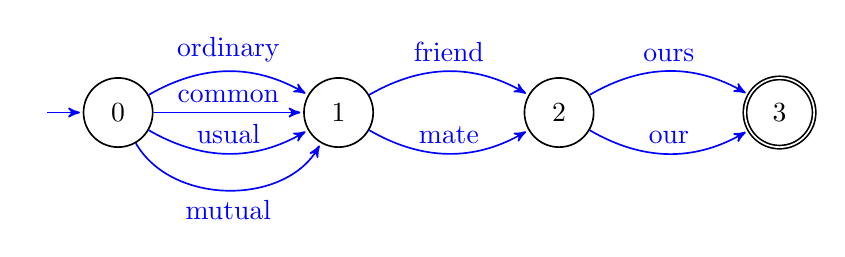
\begin{tikzpicture}[->,>=stealth',shorten >=1pt,auto,node distance=2.8cm,semithick]
\tikzstyle{every state}=[draw=black,text=black]
\tikzstyle{every path}=[draw=blue,text=blue]	

\node[initial,state,style={initial text=}] (A) {$0$};
\node[state] (B) [right of=A] {$1$};
\node[state] (C) [right of=B] {$2$};
\node[state,accepting] (D) [right of=C] {$3$};
	\path
		(A) edge node {\etext{common}} (B)
			edge [bend right] node {\etext{usual}} (B)
			edge [bend left] node {\etext{ordinary}} (B)
			edge [bend right=60] node [below] {mutual} (B)
		(B) edge [bend right] node {\etext{mate}} (C)
			edge [bend left] node {\etext{friend}} (C)
		(C) edge [bend right] node {\etext{our}} (D)
			edge [bend left] node {\etext{ours}} (D);
\end{tikzpicture} 
}
}

\end{column}
\end{columns}
	
\only<7>{$3! = 3 \times 2 \times 1 = 6$ permutations}
\only<8>{each has $2 \times 2 \times 4 = 16$ translations \\}
\only<9>{amounting to $6 \times 16 = 96$ solutions}
\only<10>{$I!$ permutations $\times$ $t^I$ translations}


}


\frame{
	\frametitle{Packing permutations}
	
	%\scalebox{0.7}{%
\begin{tikzpicture}[->,>=stealth',shorten >=1pt,auto,node distance=2.8cm,semithick]
\tikzstyle{every state}=[draw=black,text=black]
\node[initial,state,style={initial text=}] (q000) {\only<1-4>{$0$}\only<5->{$000$}};
\only<1-5>{\node[state] (q1) [right of=q000] {$1$};}
\only<1-7>{\node[state] (q2) [right of=q1] {$2$};}
\only<1-7>{\node[state,accepting] (q3) [right of=q2] {$3$};}
\only<5->{\node[state] (q100) [above right of=q000] {$100$};}
\only<6->{
\node[state] (q010) [right of=q000] {$010$};
\node[state] (q001) [below right of=q000] {$001$};
}
\only<7->{\node[state] (q110) [above of=q2] {$110$};}
\only<8->{
\node[state] (q101) [right of=q010] {$101$};
\node[state] (q011) [below of=q2] {$011$};
\node[state,accepting] (q111) [right of=q101] {$111$};
}

\only<1>{\path[color=gray,text=gray] 
(q000) edge node {nosso} (q1);}
\only<1-2>{\path[color=gray,text=gray] 
(q1) edge node {amigo} (q2);}
\only<1-3>{\path[color=gray,text=gray] 
(q2) edge node {comum} (q3);}

\only<2-4>{\path[color=red,text=red] 
(q000) edge [bend left] node {nosso} (q1);}
\only<2-5>{\path[color=red,text=red] 
(q000) edge node {amigo} (q1);}
\only<2-5>{\path[color=red,text=red] 
(q000) edge [bend right] node {comum} (q1);}


\only<3-6>{
\path[color=red,text=red] 
	(q1) edge [bend left] node {nosso} (q2);}
\only<3-5>{
\path[color=red,text=red] 
	(q1) edge node {amigo} (q2);}
\only<3-7>{
\path[color=red,text=red] 
	(q1) edge [bend right ]node {comum} (q2);}
		
\only<4-7>{
\path[color=red,text=red] 
	(q2) edge [bend left] node {nosso} (q3);}
\only<4-7>{
\path[color=red,text=red] 
	(q2) edge node {amigo} (q3);}
\only<4-6>{
\path[color=red,text=red] 
	(q2) edge [bend right ]node {comum} (q3);}
		
\only<5->{\path[color=red,text=red] 
(q000) edge [bend left] node {nosso} (q100);}

\only<5-6>{
\path[color=red,text=red] 
	(q100) edge [bend left=90] node {amigo} (q2);
}
\only<5-7>{
\path[color=red,text=red] 
	(q100) edge [bend left=30] node {comum} (q2);
}
\only<6->{\path[color=red,text=red] 
(q000) edge [bend right] node {\ftext{comum}} (q001);}
\only<6->{\path[color=red,text=red] 
(q000) edge node {amigo} (q010);}


\only<6-7>{
\path[color=red,text=red] 
(q001) edge [bend right=30] node {\ftext{nosso}} (q2);
}
\only<6-7>{
\path[color=red,text=red] 
(q001) edge [bend right=90] node [below] {\ftext{amigo}} (q2);
}
\only<7->{
\path[color=red,text=red] 
(q100) edge [bend left] node {\ftext{amigo}} (q110)
(q010) edge [bend right] node [below] {\ftext{nosso}} (q110)
(q110) edge [bend left] node {\ftext{comum}} (q3);
}
\only<8->{
\path[color=red,text=red] 
(q100) edge [bend left] node [above] {\ftext{comum}} (q101)
(q010) edge node {\ftext{comum}} (q011)
(q001) edge [bend right] node {\ftext{nosso}} (q101)
(q001) edge [bend right] node [below] {\ftext{amigo}} (q011)
(q101) edge node {\ftext{amigo}} (q111)
(q011) edge [bend right] node [below] {\ftext{nosso}} (q111);
}
\end{tikzpicture}
%}

	
}

\frame{
	\frametitle{Packing permutations}

	\begin{textblock*}{80mm}(0.5\textwidth,0.5\textheight)
	
\scalebox{0.6}{
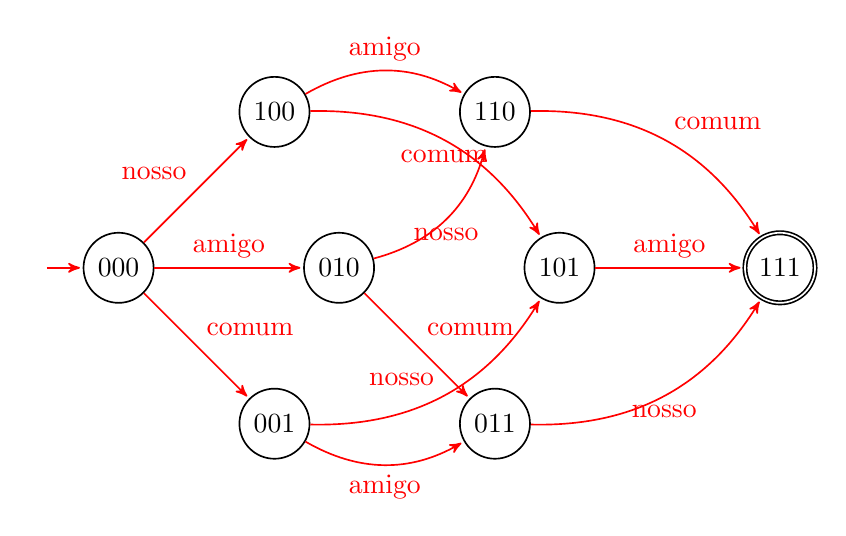
\begin{tikzpicture}[->,>=stealth',shorten >=1pt,auto,node distance=2.8cm,semithick]
\tikzstyle{every state}=[draw=black,text=black]
\tikzstyle{every path}=[draw=red,text=red]

\node[initial,state,style={initial text=}] (q000) {$000$};
\node[state] (q100) [above right of=q000] {$100$};
\node[state] (q010) [right of=q000] {$010$};
\node[state] (q001) [below right of=q000] {$001$};
\node[state] (q110) [above right of=q010] {$110$};
\node[state] (q101) [right of=q010] {$101$};
\node[state] (q011) [below right of=q010] {$011$};
\node[state,accepting] (q111) [right of=q101] {$111$};

\path 
(q000) edge node {\ftext{nosso}} (q100)
(q000) edge node {\ftext{amigo}} (q010)
(q000) edge node {\ftext{comum}} (q001)
%
(q100) edge [bend left] node {\ftext{amigo}} (q110)
(q100) edge [bend left] node [below] {\ftext{comum}} (q101)
%
(q110) edge [bend left] node {\ftext{comum}} (q111)
%
(q010) edge [bend right] node [below] {\ftext{nosso}} (q110)
(q010) edge node {\ftext{comum}} (q011)
%
(q001) edge [bend right] node {\ftext{nosso}} (q101)
(q001) edge [bend right] node [below] {\ftext{amigo}} (q011)
%
(q101) edge node {\ftext{amigo}} (q111)
%
(q011) edge [bend right] node [below] {\ftext{nosso}} (q111);

\end{tikzpicture} 
}

	\end{textblock*}
	

%	Each state represents a set in the powerset of $\{1,2,\ldots, I\}$\\
	Powerset (\emph{all subsets}) of $\{1, 2, \ldots, I\}$
	\begin{itemize}
		\item $2^I$ subsets \\
		think of a vector of $I$ bits ;)
	\end{itemize}
	Lattice
	\begin{itemize}
		\item $O(2^I)$ states
		\item $O(I\times 2^I)$ transitions
	\end{itemize}	
	
	
}

%\begin{comment}
\frame{
	\frametitle{Deductive logic}
	
	
	\begin{columns}
	\begin{column}{0.4\linewidth}
	
\newcommand{\powersetcond}{
\begin{array}{l }
\textcolor<4>{ForestGreen}{1 \leq i \leq I} \\
\textcolor<4>{Red}{c_i = \bzero}
\end{array}
}



\begin{math} %\small
 \left. 
  \begin{array}{l}
    \alert<2>{\textsc{Item}} ~~~~ {\itembrack{\textcolor<2>{blue}{\{0,1\}^I}}} \\
    %\\
    \alert<5>{\textsc{Goal}} ~~~~ {\textcolor<5>{blue}{\itembrack{1^I}}} \\
    %\\  
    \alert<3>{\textsc{Axiom}} \\ 
	\drule{}{\itembrack{\textcolor<3>{blue}{0^I}}}{} \\
    %\\  
    \alert<4>{\textsc{Expand}} \\ 
	\drule{\textcolor<4>{blue}{\itembrack{C}}}{\textcolor<4>{Fuchsia}{\itembrack{\alpha_i(C)}}}{\powersetcond} \\ 
	~~ \text{\small where $\alpha_i(C)$ is a copy of $C$ with $c_i = \bone$}

  \end{array} 
\right.
\end{math}


	\end{column}
	\begin{column}{0.6\linewidth}
		\only<1>{
		Template
		\begin{itemize}
			\item items \ra states
			\item deduction rules \ra transitions
		\end{itemize}
		}
		\only<2>{
		\begin{itemize}
			\item a subset of $\{1, \ldots, I\}$\\
			encoded as a \textcolor{blue}{bit vector of length $I$}
			
		\end{itemize}
		}
		\only<3>{
		\begin{itemize}
			\item we start with an empty sentence \\
			e.g. $I=3 \ra 0^3 = \textcolor{blue}{000}$ 
		\end{itemize}
		}
		\only<4>{
		\begin{itemize}
			\item and continue one word at a time\\
			e.g. $\textcolor{blue}{\itembrack{\textcolor{Red}{0}00}} \textcolor{ForestGreen}{(i=1)} \ra \textcolor{Fuchsia}{\itembrack{100}}$ \\
		\end{itemize}
		}
		\only<5>{
		\begin{itemize}
			\item until we have a complete sentence\\
			e.g. \textcolor<5>{blue}{$\itembrack{111}$}
		\end{itemize}
		}

	\end{column}
	\end{columns}
}
%\end{comment}


%\begin{comment}
\frame{
	\frametitle{Instantiated deductive logic program}
	
	\begin{textblock*}{80mm}(0.7\textwidth,0.15\textheight)
	\scalebox{0.8}{
\newcommand{\powersetbcond}{
\begin{array}{l }
1 \leq i \leq I \\
\textcolor<6,10,14>{BurntOrange}{
	c_i = \bzero
}
\end{array}
}



\begin{math} %\small
 \left. 
  \begin{array}{l}
    \textsc{Item} ~~~~ {\itembrack{\{0,1\}^I}} \\
    %\\
    \alert<19>{\textsc{Goal}} ~~~~ {\textcolor<19>{red}{\itembrack{1^I}}} \\
    %\\  
    \alert<2>{\textsc{Axiom}} \\ 
	\drule{}{\itembrack{\textcolor<2>{blue}{0^I}}}{} \\
    %\\  
    \alert<3-18>{\textsc{Expand}} \\ 
	\drule{%
		\textcolor<18>{Magenta}{
		\textcolor<17>{Orange}{
		\textcolor<16>{Goldenrod}{
		\textcolor<12-14>{ForestGreen}{
		\textcolor<9-11>{ProcessBlue}{
		\textcolor<6-8>{Fuchsia}{
		\textcolor<3-5>{blue}{
			\itembrack{C}
		}}}}}}}
	}%
	{%
		\textcolor<16-18>{red}{
		\textcolor<11,13>{Magenta}{
		\textcolor<9>{Goldenrod}{
		\textcolor<8,12>{Orange}{
		\textcolor<7>{Goldenrod}{
		\textcolor<5>{ForestGreen}{
		\textcolor<4>{ProcessBlue}{
		\textcolor<3>{Fuchsia}{
			\itembrack{\alpha_i(C)}
		}}}}}}}}
	}%
	{\powersetbcond} \\ 
	%~~ \text{\small where $\alpha_i(C)$ is a copy of $C$ with $c_i = \bone$}

  \end{array} 
\right.
\end{math}

}
	\end{textblock*}
	
	\begin{small}
		Source: \ftext{nosso}$_1$ \ftext{amigo}$_2$ \ftext{comum}$_3$ \\
	\only<2->{
	\texttt{Axiom} \\
	~ {\color{blue}\itembrack{000}} \\
	}
	\only<3->{
	\texttt{Expand} \\
	~ ${\color{blue}\itembrack{000} }(i=1) \ra {\color{Fuchsia}\itembrack{100}}$  \\
	}
	\only<4->{
	~ ${\color{blue}\itembrack{000}} (i=2) \ra {\color{ProcessBlue}\itembrack{010}}$  \\
	}
	\only<5->{
	~ ${\color{blue}\itembrack{000}} (i=3) \ra {\color{ForestGreen}\itembrack{001}}$  \\
	}
	\only<6-14>{
	~ ${\color{Fuchsia}\itembrack{100}} (i=1)$ \xmark  \\
	}
	\only<7->{
	~ ${\color{Fuchsia}\itembrack{100}} (i=2) \ra {\color{Goldenrod}\itembrack{110}}$  \\
	}
	\only<8->{
	~ ${\color{Fuchsia}\itembrack{100}} (i=3) \ra {\color{Orange}\itembrack{101}}$  \\
	}
	\only<9->{
	~ ${\color{ProcessBlue}\itembrack{010}} (i=1) \ra {\color{Goldenrod}\itembrack{110}} $  \\
	}
	\only<10-14>{
	~ ${\color{ProcessBlue}\itembrack{010}} (i=2)$ \xmark \\
	}
	\only<11->{
	~ ${\color{ProcessBlue}\itembrack{010}} (i=3) \ra {\color{Magenta}\itembrack{011}}$  \\
	}
	\only<12->{
	~ ${\color{ForestGreen}\itembrack{001}} (i=1) \ra {\color{Orange}\itembrack{101}} $  \\
	}
	\only<13->{
	~ ${\color{ForestGreen}\itembrack{001}} (i=2) \ra {\color{Magenta}\itembrack{011}} $  \\
	}
	\only<14>{
	~ ${\color{ForestGreen}\itembrack{001}} (i=3)$ \xmark \\
	}
	%\only<15->{
	%~ ${\color{Goldenrod}\itembrack{110}} (i=1..2)$ \xmark \\
	%}
	\only<16->{
	~ ${\color{Goldenrod}\itembrack{110}} (i=3) \ra {\color{red}\itembrack{111}}$ \\
	}
	%\only<17->{
	%~ ${\color{Orange}\itembrack{101}} (i=1,3)$ \xmark \\
	%}
	\only<17->{
	~ ${\color{Orange}\itembrack{101}} (i=2) \ra {\color{red}\itembrack{111}}$  \\
	}
	\only<18->{
	~ ${\color{Magenta}\itembrack{011}} (i=1) \ra {\color{red}\itembrack{111}}$  \\
	}
	%\only<20->{
	%~ ${\color{Magenta}\itembrack{011}} (i=2,3) $  \xmark \\
	%}
	\only<19>{
	\texttt{Goal} \\
	~ {\color{red}\itembrack{111}} \\
	}
	\end{small}
	
	\begin{textblock*}{80mm}(0.45\textwidth,0.5\textheight)
		\scalebox{0.6}{\begin{tikzpicture}[->,>=stealth',shorten >=1pt,auto,node distance=2.8cm,semithick]
\tikzstyle{every state}=[draw=black]
\tikzstyle{every path}=[draw=red,text=red]

\only<2->{\node[initial,state,style={initial text=},text=blue] (q000) {$000$};}
\only<3->{\node[state] (q100) [above right of=q000,text=Fuchsia] {$100$};}
\only<4->{\node[state] (q010) [right of=q000,text=ProcessBlue] {$010$};}
\only<5->{\node[state] (q001) [below right of=q000,text=ForestGreen] {$001$};}
\only<7->{\node[state] (q110) [above right of=q010,text=Goldenrod] {$110$};}
\only<8->{\node[state] (q101) [right of=q010,text=Orange] {$101$};}
\only<11->{\node[state] (q011) [below right of=q010,text=Magenta] {$011$};}
\only<16->{\node[state,accepting] (q111) [right of=q101,text=red] {$111$};}

\only<3->{\path (q000) edge node {\ftext{nosso}} (q100);}
\only<4->{\path (q000) edge node {\ftext{amigo}} (q010);}
\only<5->{\path (q000) edge node {\ftext{comum}} (q001);}
%
\only<7->{\path (q100) edge [bend left] node {\ftext{amigo}} (q110);}
\only<8->{\path (q100) edge [bend left] node [below] {\ftext{comum}} (q101);}
%
%
\only<9->{\path (q010) edge [bend right] node [below] {\ftext{nosso}} (q110);}
\only<11->{\path (q010) edge node {\ftext{comum}} (q011);}
%
\only<12->{\path (q001) edge [bend right] node {\ftext{nosso}} (q101);}
\only<13->{\path (q001) edge [bend right] node [below] {\ftext{amigo}} (q011);}
%
\only<16->{\path (q110) edge [bend left] node {\ftext{comum}} (q111);}
%
\only<17->{\path (q101) edge node {\ftext{amigo}} (q111);}
%
\only<18->{\path (q011) edge [bend right] node [below] {\ftext{nosso}} (q111);}

\end{tikzpicture} }
	\end{textblock*}

}
%\end{comment}

\frame{
	\frametitle{Word replacement with unconstrained reordering}
	
	
	
	\only<2>{
	\begin{textblock*}{100mm}(0.1\textwidth,0.2\textheight)
	\scalebox{1.2}{
	
\scalebox{0.6}{
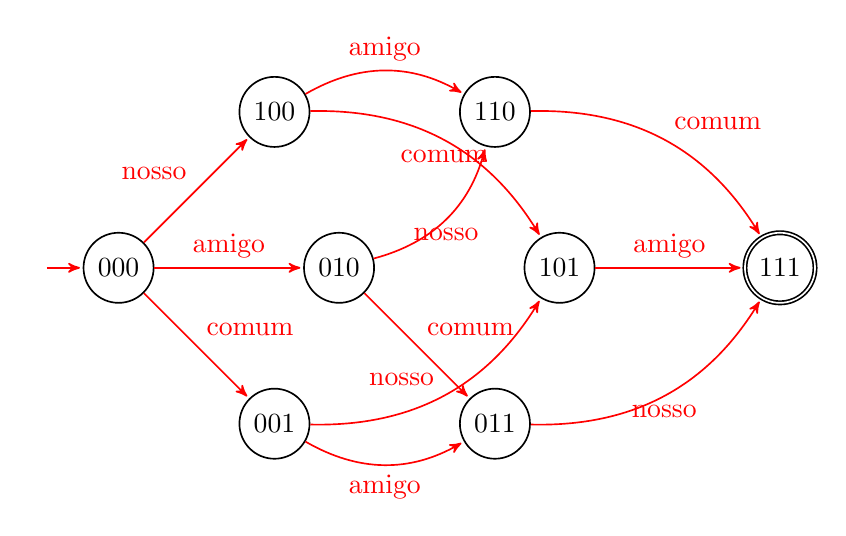
\begin{tikzpicture}[->,>=stealth',shorten >=1pt,auto,node distance=2.8cm,semithick]
\tikzstyle{every state}=[draw=black,text=black]
\tikzstyle{every path}=[draw=red,text=red]

\node[initial,state,style={initial text=}] (q000) {$000$};
\node[state] (q100) [above right of=q000] {$100$};
\node[state] (q010) [right of=q000] {$010$};
\node[state] (q001) [below right of=q000] {$001$};
\node[state] (q110) [above right of=q010] {$110$};
\node[state] (q101) [right of=q010] {$101$};
\node[state] (q011) [below right of=q010] {$011$};
\node[state,accepting] (q111) [right of=q101] {$111$};

\path 
(q000) edge node {\ftext{nosso}} (q100)
(q000) edge node {\ftext{amigo}} (q010)
(q000) edge node {\ftext{comum}} (q001)
%
(q100) edge [bend left] node {\ftext{amigo}} (q110)
(q100) edge [bend left] node [below] {\ftext{comum}} (q101)
%
(q110) edge [bend left] node {\ftext{comum}} (q111)
%
(q010) edge [bend right] node [below] {\ftext{nosso}} (q110)
(q010) edge node {\ftext{comum}} (q011)
%
(q001) edge [bend right] node {\ftext{nosso}} (q101)
(q001) edge [bend right] node [below] {\ftext{amigo}} (q011)
%
(q101) edge node {\ftext{amigo}} (q111)
%
(q011) edge [bend right] node [below] {\ftext{nosso}} (q111);

\end{tikzpicture} 
}

	}
	\end{textblock*}
	}
	
	\only<3>{
	\begin{textblock*}{100mm}(0.1\textwidth,0.1\textheight)
	\scalebox{0.9}{
	
\scalebox{0.6}{
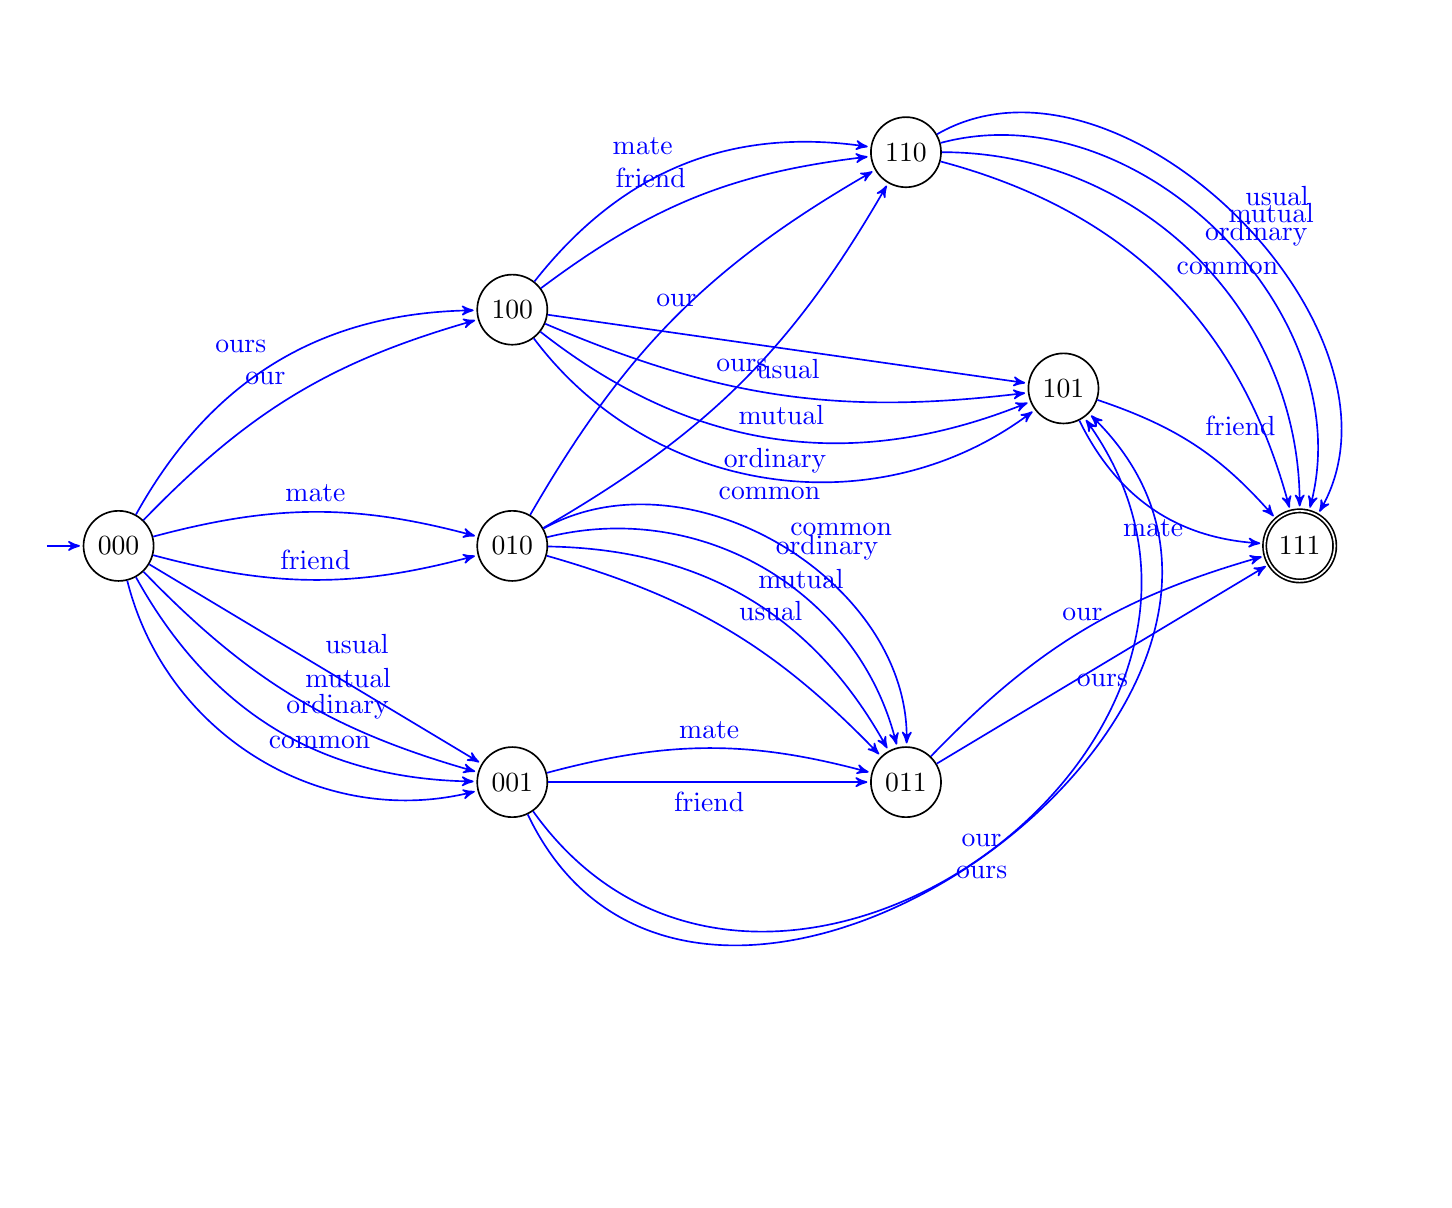
\begin{tikzpicture}[->,>=stealth',shorten >=1pt,auto,node distance=2.8cm,semithick]
\tikzstyle{every state}=[draw=black,text=black]
\tikzstyle{every path}=[draw=blue,text=blue]

\node[initial,state,style={initial text=}] (q000) at (0,-3) {$000$};
\node[state] (q100) at (5,0) {$100$};
\node[state] (q010) at (5,-3) {$010$};
\node[state] (q001) at (5,-6) {$001$};
\node[state] (q110) at (10,2) {$110$};
\node[state] (q101) at (12,-1) {$101$};
\node[state] (q011) at (10,-6) {$011$};
\node[state,accepting] (q111) at (15,-3) {$111$};

\path 
(q000) edge [bend left=15] node {\etext{our}} (q100)
(q000) edge [bend left=30] node {\etext{ours}} (q100)

(q000) edge [bend left=15] node {\etext{mate}} (q010)
(q000) edge [bend right=15] node {\etext{friend}} (q010)

(q000) edge  node {\etext{usual}} (q001)
(q000) edge [bend right=15] node {\etext{mutual}} (q001)
(q000) edge [bend right=30] node {\etext{ordinary}} (q001)
(q000) edge [bend right=45] node {\etext{common}} (q001)

%
(q100) edge [bend left=15] node {\etext{friend}} (q110)
(q100) edge [bend left=30] node {\etext{mate}} (q110)

(q100) edge node [below] {\etext{usual}} (q101)
(q100) edge [bend right=15] node [below] {\etext{mutual}} (q101)
(q100) edge [bend right=30] node [below] {\etext{ordinary}} (q101)
(q100) edge [bend right=45] node [below] {\etext{common}} (q101)

%
(q110) edge [bend left=75] node {\etext{usual}} (q111)
(q110) edge [bend left=60] node {\etext{mutual}} (q111)
(q110) edge [bend left=45] node {\etext{ordinary}} (q111)
(q110) edge [bend left=30]node {\etext{common}} (q111)

%
(q010) edge [bend left=15] node [above] {\etext{our}} (q110)
(q010) edge [bend right=15] node [above] {\etext{ours}} (q110)

(q010) edge [bend left=15] node {\etext{usual}} (q011)
(q010) edge [bend left=30] node {\etext{mutual}} (q011)
(q010) edge [bend left=45] node {\etext{ordinary}} (q011)
(q010) edge [bend left=60] node {\etext{common}} (q011)
%
(q001) edge [bend right=90,looseness=1.5] node [above] {\etext{our}} (q101)
(q001) edge [bend right=100,looseness=1.5] node [below] {\etext{ours}} (q101)
(q001) edge node [below] {\etext{friend}} (q011)
(q001) edge [bend left=15] node [above] {\etext{mate}} (q011)
%
(q101) edge [bend left=15] node {\etext{friend}} (q111)
(q101) edge [bend right] node [below] {\etext{mate}} (q111)
%
(q011) edge [bend left=15] node [above] {\etext{our}} (q111)
(q011) edge node [below] {\etext{ours}} (q111);

\end{tikzpicture} 
}

	}
	\end{textblock*}
	}

	\begin{textblock*}{100mm}(0.1\textwidth,0.8\textheight)	
	\small
	Source: \ftext{nosso amigo comum} 
	\begin{enumerate}
		\item<2-> arbitrary permutations: $O(2^I)$ states
		\item<3-> intersection with the rule set:  $O(tI2^I)$ transitions
	\end{enumerate}
	\end{textblock*}
}


\frame{
	\frametitle{Problem!}
	
	Before we even discuss a parameterisation of the model we already ran into a tractability issue!
	\pause
	\begin{itemize}
		\item NP-complete \citep{Knight:1999:tsp}
		\item generalised TSP
	\end{itemize}
	\pause
	Direction
	\begin{itemize}
		\item is it sensible to consider the space of {\bf all permutations}?
	\end{itemize}
	\pause
	Solution
	\pause
	\begin{itemize}
		\item constrain reordering {\bf :D}
		\pause
		\item {\bf 0.o} but how?
	\end{itemize}
}


	\subsection{Distortion limit}

\frame{
	\frametitle{Ad-hoc distortion limit}
	
	Several flavours of distortion limit \citep{Lopez:2009:TWD}
	\pause
	\begin{itemize}
		\item limit reordering as a function of the number of skipped words
	\end{itemize}
	\pause
	Moses allows reordering within a window of length $d$
	\begin{itemize}
		\item starting from the leftmost uncovered word
	\end{itemize}
	
}

\begin{comment}
\frame{
	\frametitle{WL$d$ (intuition)}
	Suppose a sentence with $I=6$ words and $d=3$\\
	
	~
	
	\textcolor{gray}{
	\begin{tabular}{|c | c | c | c | c | c |}
	\hline
	\textcolor{black}{1} & \textcolor{black}{2} & \textcolor{black}{3} & \textcolor{black}{4} & \textcolor{black}{5} & \textcolor{black}{6} \\ \hline
	\textcolor{red}{0} & \textcolor{blue}{\only<2-3>{0}\only<4-5>{1}} & \textcolor{blue}{\only<2,5>{0}\only<3-4>{1}}  & 0 & 0 & 0 \\
	1 & \textcolor{red}{0} & \textcolor{blue}{\only<6-7>{0}\only<8-9>{1}}  & \textcolor{blue}{\only<6,9>{0}\only<7-8>{1}} & 0 & 0 \\
	1 & 1 & \textcolor{red}{0} & \textcolor{blue}{\only<10-11>{0}\only<12-13>{1}} & \textcolor{blue}{\only<10,13>{0}\only<11-12>{1}} & 0 \\
	1 & 1 & 1 & \textcolor{red}{0} & \textcolor{blue}{\only<14-15>{0}\only<16-17>{1}} & \textcolor{blue}{\only<14,17>{0}\only<15-16>{1}} \\
	1 & 1 & 1 & 1 & \textcolor{red}{0} & \textcolor{blue}{\only<18>{0}\only<19>{1}} \\
	1 & 1 & 1 & 1 & 1 & \textcolor{red}{0} \\	
	1 & 1 & 1 & 1 & 1 & 1 \\		
	\hline
	\end{tabular}
	}
	
	~
	
	
	\only<20>{
	Largely reduced set of permutations
	\begin{itemize}
		\item $(I-1)2^{d-1}$ configurations
	\end{itemize}
	}
}
\end{comment}


\frame{
	\frametitle{WL$d$ (example)}
	
	Suppose $d=2$ and $I=3$ 
	\only<10>{(e.g. \ftext{nosso amigo comum})} \\

~


\scalebox{0.8}{
\begin{tikzpicture}[->,>=stealth',shorten >=1pt,auto,node distance=2.8cm,semithick]
\tikzstyle{every state}=[draw=black,text=black]
\tikzstyle{every path}=[draw=red,text=red]

\only<2->{\node[initial,state,style={initial text=}] (q10) {$[1,2]$};}
\only<3->{\node[state] (q20) [above right of=q10] {$[2,3]$};}
\only<4->{\node[state] (q11) [below right of=q10] {$[1,\not2]$};}
\only<5->{\node[state] (q3) [right of=q11] {$[3 ]$};}
\only<7->{\node[state] (q21) [right of=q20] {$[2,\not3]$};}
\only<8->{\node[state,accepting] (q4) [below right of=q21] {$\varnothing$};}



\only<3-9>{\path (q10) edge node {\ftext{1}} (q20);}
\only<4-9>{\path (q10) edge node {\ftext{2}} (q11);}
\only<5-9>{\path (q11) edge node {\ftext{1}} (q3);}
\only<6-9>{\path (q20) edge node {\ftext{2}} (q3);}
\only<7-9>{\path (q20) edge node {\ftext{3}} (q21);}
\only<8-9>{\path (q21) edge node {\ftext{2}} (q4);}
\only<9>{\path (q3) edge node {\ftext{3}} (q4);}

\only<10>{
\path (q10) edge node {\ftext{nosso}} (q20);
\path (q10) edge node {\ftext{amigo}} (q11);
\path (q20) edge node {\ftext{comum}} (q21);
\path (q20) edge node {\ftext{amigo}} (q3);
\path (q11) edge node {\ftext{nosso}} (q3);
\path (q3) edge node {\ftext{comum}} (q4);
\path (q21) edge node {\ftext{amigo}} (q4);
}



\end{tikzpicture} 
}


	
}



\frame{
	\frametitle{WL$d$ (logic)}
	
	
	\begin{columns}
	\begin{column}{0.4\linewidth}
	
\newcommand{\wldadjcond}{
\begin{array}{l }
i = l\\
\end{array}
}

\newcommand{\wldnonadjcond}{
\begin{array}{l }
l < i \leq I \\
\delta(i, l) \leq d \\
c_{i-l} = \bzero \\
\end{array}
}


\begin{math} %\small
 \left. 
  \begin{array}{l}
    \textsc{Item} ~~~~ {\itembrack{[1 .. I +1], \{0,1\}^{d-1}}} \\
    %\\
    \textsc{Goal} ~~~~ {\itembrack{I+1, C}} \\
    %\\  
    \textsc{Axiom} \\ 
	\drule{}{\itembrack{1, 0^{d-1}}}{} \\
    %\\  
    \textsc{Adjacent} \\ 
	\drule{\itembrack{l, C}}{\itembrack{l + n, C \ll n}}{\wldadjcond} \\ 
	~~ \text{\small where $n = \#_1(C) + 1$} \\
%	~~ \text{\small and $\#_1(C)$ is the number of leading ones in $C$} \\
    \textsc{Non-Adjacent} \\ 
	\drule{\itembrack{l, C}}{\itembrack{l, \alpha_l^{i}(C)}}{\wldnonadjcond} \\ 
	
  \end{array} 
\right.
\end{math}


	\end{column}
	\begin{column}{0.6\linewidth}
		
	\begin{itemize}
		\item $O(Id2^{d-1})$ states
		\item $O(Id2^{d-1})$ transitions
	\end{itemize}

	\end{column}
	\end{columns}
}



\frame{
	\frametitle{Word replacement with reordering constrained by WL$2$}
	
	\only<1>{Complexity: $O(I2^{d-1})$ states\\}
	\only<2>{Complexity: $O(tI2^{d-1})$ transitions\\}	

~

\scalebox{0.8}{
\begin{tikzpicture}[->,>=stealth',shorten >=1pt,auto,node distance=2.8cm,semithick]
\tikzstyle{every state}=[draw=black,text=black]

\node[initial,state,style={initial text=}] (q10) {$[1,2]$};
\node[state] (q20) [above right of=q10] {$[2,3]$};
\node[state] (q11) [below right of=q10] {$[1,\not2]$};
\node[state] (q3) [right of=q11] {$[3 ]$};
\node[state] (q21) [right of=q20] {$[2,\not3]$};
\node[state,accepting] (q4) [below right of=q21] {$\varnothing$};

\only<1>{
\path[draw=red] (q10) edge node {\ftext{nosso}} (q20)
	(q10) edge node {\ftext{amigo}} (q11)
	(q20) edge node {\ftext{comum}} (q21)
	(q20) edge node {\ftext{amigo}} (q3)
	(q11) edge node {\ftext{nosso}} (q3)
	(q3) edge node {\ftext{comum}} (q4)
	(q21) edge node {\ftext{amigo}} (q4);
}

\only<2>{
\path[draw=blue] (q10) edge [bend left=15] node [above] {\etext{our}} (q20)
	(q10) edge  node [below] {\etext{ours}} (q20)

	(q10) edge node [above] {\etext{friend}} (q11)
	(q10) edge [bend right=15] node [below] {\etext{mate}} (q11)

	(q20) edge [bend left=45] node [above] {\etext{ordinary}} (q21)
	(q20) edge [bend left=30] node {\etext{mutual}} (q21)
	(q20) edge node {\etext{common}} (q21)
	(q20) edge [bend right=15] node {\etext{usual}} (q21)			

	(q20) edge [bend left=15] node {\etext{friend}} (q3)
	(q20) edge [bend right=15] node {\etext{mate}} (q3)

	(q11) edge node {\etext{our}} (q3)
	(q11) edge [bend right=15] node [below] {\etext{ours}} (q3)

	(q3) edge node {\etext{usual}} (q4)
	(q3) edge [bend right=15] node {\etext{mutual}} (q4)
	(q3) edge [bend right=30] node [below] {\etext{common}} (q4)
	(q3) edge [bend right=45] node [below] {\etext{ordinary}} (q4)			

	(q21) edge [bend left=30] node [above] {\etext{friend}} (q4)
	(q21) edge node {\etext{mate}} (q4);

}

\end{tikzpicture} 
}

	
}


	\frame{
	\frametitle{Ad-hoc distortion limit: expressiveness}
	
	Arbitrarily limit reordering to a fixed-length window \pause
	\begin{itemize}
		\item conveniently (linear complexity), but \pause
		\item what about languages with very different syntax? \\
		e.g. OV vs VO, head-initial vs head-final \pause
		\item can we do better?
	\end{itemize}
	
}

\frame{
	\frametitle{Binary permutations}
	
	Consider a sentence such that $I=4$ \\
	~ let's look at binary trees bracketing this sentence\\ \pause

\scalebox{0.9}{
\textcolor<3-10>{ForestGreen}{
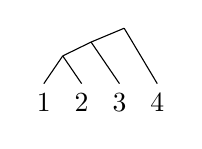
\begin{tikzpicture}[level distance=5pt]
\tikzset{frontier/.style={distance from root=30pt}}
\Tree 
[
	[ 
		[ 1 2 ]
		3
	]
	4
]
\end{tikzpicture}
}
~
\textcolor<11>{ForestGreen}{
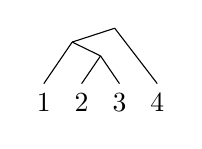
\begin{tikzpicture}[level distance=5pt]
\tikzset{frontier/.style={distance from root=30pt}}
\Tree 
[
	[ 
		1
		[ 2 3 ]
	]
	4
]
\end{tikzpicture}
}
~ 
\textcolor<12>{ForestGreen}{
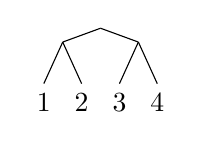
\begin{tikzpicture}[level distance=5pt]
\tikzset{frontier/.style={distance from root=30pt}}
\Tree 
[
	[ 1 2 ]
	[ 3 4 ]
]
\end{tikzpicture}
}
~
\textcolor<13>{ForestGreen}{
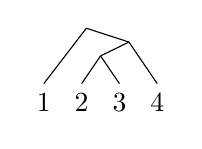
\begin{tikzpicture}[level distance=5pt]
\tikzset{frontier/.style={distance from root=30pt}}
\Tree 
[
	1
	[ 
		[ 2 3 ]
		4
	]
]
\end{tikzpicture}
}
~
\textcolor<14>{ForestGreen}{
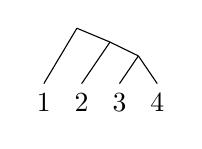
\begin{tikzpicture}[level distance=5pt]
\tikzset{frontier/.style={distance from root=30pt}}
\Tree 
[
	1
	[ 
		2
		[ 3 4 ]
	]
]
\end{tikzpicture}
}
}

	\only<3->{Binary permutations\\} 
\only<3-10>{
\begin{tabular}{l l}
\only<3-10>{\dbr{\dbr{\dbr{1 2}3}4} & 1 2 3 4 }\\
\only<4-10>{\dbr{\dbr{\ibr{1 2}3}4} & 2 1 3 4 }\\
\only<5-10>{\dbr{\ibr{\dbr{1 2}3}4} & 3 1 2 4 }\\
\only<6-10>{\dbr{\ibr{\ibr{1 2}3}4} & 3 2 1 4 }\\
\only<7-10>{\ibr{\dbr{\dbr{1 2}3}4} & 4 1 2 3 }\\
\only<8-10>{\ibr{\dbr{\ibr{1 2}3}4} & 4 2 1 3 }\\
\only<9-10>{\ibr{\ibr{\dbr{1 2}3}4} & 4 3 1 2 }\\
\only<10-10>{\ibr{\ibr{\ibr{1 2}3}4} & 4 3 2 1 }\\ 
\end{tabular}
}

\only<11>{
\begin{tabular}{l l}
\dbr{\dbr{1\dbr{2 3}}4} & 1 2 3 4 \\
\dbr{\dbr{1\ibr{2 3}}4} & 1 3 2 4 \\
\dbr{\ibr{1\dbr{2 3}}4} & 2 3 1 4 \\
\dbr{\ibr{1\ibr{2 3}}4} & 3 2 1 4 \\
\ibr{\dbr{1\dbr{2 3}}4} & 4 1 2 3 \\
\ibr{\dbr{1\ibr{2 3}}4} & 4 1 3 2 \\
\ibr{\ibr{1\dbr{2 3}}4} & 4 2 3 1 \\
\ibr{\ibr{1\ibr{2 3}}4} & 4 3 2 1 \\ 
\end{tabular}
}

\only<12>{
\begin{tabular}{l l}
\dbr{\dbr{1 2}\dbr{3 4}} & 1 2 3 4\\
\dbr{\ibr{1 2}\dbr{3 4}} & 2 1 3 4\\
\dbr{\ibr{1 2}\ibr{3 4}} & 2 1 4 3 \\
\dbr{\dbr{1 2}\ibr{3 4}} & 1 2 4 3 \\
\ibr{\dbr{1 2}\dbr{3 4}} & 3 4 1 2 \\
\ibr{\ibr{1 2}\dbr{3 4}} & 3 4 2 1 \\
\ibr{\ibr{1 2}\ibr{3 4}} & 4 3 2 1 \\
\ibr{\dbr{1 2}\ibr{3 4}} & 4 3 1 2 \\
\end{tabular}
}

\only<13>{
\begin{tabular}{l l}
\dbr{1\dbr{\dbr{2 3}4}} & 1 2 3 4 \\
\dbr{1\dbr{\ibr{2 3}4}} & 1 3 2 4 \\
\dbr{1\ibr{\dbr{2 3}4}} & 1 4 2 3 \\
\dbr{1\ibr{\ibr{2 3}4}} & 1 4 3 2 \\
\ibr{1\dbr{\dbr{2 3}4}} & 2 3 4 1 \\
\ibr{1\dbr{\ibr{2 3}4}} & 3 2 4 1 \\
\ibr{1\ibr{\dbr{2 3}4}} & 4 2 3 1 \\
\ibr{1\ibr{\ibr{2 3}4}} & 4 3 2 1 \\
\end{tabular}
}

\only<14>{
\begin{tabular}{l l}
\dbr{1\dbr{2\dbr{3 4}}} & 1 2 3 4 \\
\dbr{1\dbr{2\ibr{3 4}}} & 1 2 4 3 \\
\dbr{1\ibr{2\dbr{3 4}}} & 1 3 4 2 \\
\dbr{1\ibr{2\ibr{3 4}}} & 1 4 3 2 \\
\ibr{1\dbr{2\dbr{3 4}}} & 2 3 4 1 \\
\ibr{1\dbr{2\ibr{3 4}}} & 2 4 3 1 \\
\ibr{1\ibr{2\dbr{3 4}}} & 3 4 2 1 \\
\ibr{1\ibr{2\ibr{3 4}}} & 4 3 2 1 \\
\end{tabular}
}

\only<15->{
	\begin{itemize}
		\item<14-> constrains the space of permutations
		\item<15-> crossing constraint (shares a linguistic intuition)\\
		~ 3 1 4 2 \\
		~ 2 4 1 3 \\
	\end{itemize}
}
}


\frame{
	\frametitle{ITGs}
	
	Inversion Transduction Grammars (ITGs) \precite{Wu, 1997} \\
	\pause
	\begin{itemize}
		\item $X \ra X X$ \\
		\textcolor{blue}{direct order} \pause
		\item $X \ra \angbrack{X X}$\\
		\textcolor{red}{inverted order} \pause
		\item $X \ra f/e$, where $(f,e) \in R$\\
		\textcolor{ForestGreen}{bilingual mappings}
	\end{itemize}
	
}

\frame{
	\frametitle{Parsing, intersection and hypergraphs}

\only<1->{	
\begin{textblock*}{80mm}(0.1\textwidth,0.15\textheight)
Source\\
\scalebox{0.6}{
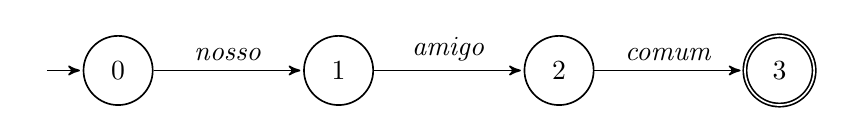
\begin{tikzpicture}[->,>=stealth',shorten >=1pt,auto,node distance=2.8cm,semithick]
%\tikzstyle{every state}=[draw=black,text=black]
%\tikzstyle{every path}=[draw=red,text=red]

\node[initial,state,style={initial text=}] (q0) {$0$};
\node[state] (q1) [right of=q0] {$1$};
\node[state] (q2) [right of=q1] {$2$};
\node[state,accepting] (q3) [right of=q2] {$3$};

\path (q0) edge node {\textit{nosso}} (q1);
\path (q1) edge node {\textit{amigo}} (q2);
\path (q2) edge node {\textit{comum}} (q3);
\end{tikzpicture}
}
\end{textblock*}
}

\only<2->{
\begin{textblock*}{80mm}(0.7\textwidth,0.15\textheight)
\footnotesize
Grammar\\
\begin{tabular}{l l}
$X \ra X X$ & \only<7-10>{\textcolor{blue}{$\Longleftarrow$}}\\
$X \ra \angbrack{X X}$ & \only<11-14>{\textcolor{red}{$\Longleftarrow$}}\\
$X \ra \textit{nosso}$ & \only<4>{\textcolor{ForestGreen}{$\Longleftarrow$}} \\ % /\{\etext{our}, \etext{ours}\}$ \\
$X \ra \textit{amigo}$ & \only<5>{\textcolor{ForestGreen}{$\Longleftarrow$}} \\ % /\{\etext{friend}, \etext{mate}\}$ \\
$X \ra \textit{comum}$ & \only<6>{\textcolor{ForestGreen}{$\Longleftarrow$}}\\ % /\{\etext{ordinary}, \etext{common}, \etext{usual}\}$ \\
\end{tabular}
\end{textblock*}
}

\only<3->{
\begin{textblock*}{80mm}(0.1\textwidth,0.3\textheight)
Intersection \\
\begin{itemize}
	\item \textcolor<4->{ForestGreen}{$_iX_j \ra f$} \\
	{\small s.t. $\angbrack{i,f,j} \in E$}
	\item \textcolor<7->{blue}{$_iX_k \ra {}_iX_j ~ {}_jX_k$} \\
	{\small s.t. $(i,j,k) \in Q^3$}
	\item \textcolor<11->{red}{$_iX_k \ra {}_jX_k ~ {}_iX_j$} \\
	{\small s.t. $(i,j,k) \in Q^3$}
\end{itemize}
\end{textblock*}
}

\begin{textblock*}{80mm}(0.45\textwidth,0.45\textheight)
\scalebox{0.8}{
\begin{tikzpicture}[->,>=stealth',thick]

\coordinate (c01) at (-1,0);
\only<4->{\node[state] (X01) at (1,0) {$_0X_1$};}
\coordinate (c02) at (2,0);
\coordinate (i02) at (2.2,-0.15);
\only<7->{\node[state] (X02) at (4,0) {$_0X_2$};}
\coordinate (c12) at (-1,-2);
\only<5->{\node[state] (X12) at (1,-2) {$_1X_2$};}
\coordinate (c23) at (-1,-4);
\only<6->{\node[state] (X23) at (1,-4) {$_2X_3$};}
\coordinate (c13) at (2,-3);
\coordinate (i13) at (1.95,-3.25);
\only<8->{\node[state] (X13) at (3,-3) {$_1X_3$};}
\coordinate (c03) at (5,0);
\coordinate (i03) at (4.9,-0.2);
\only<9->{\node[state,accepting] (X03) at (7,0) {$_0X_3$};}
\coordinate (c03b) at (4,-1);
\coordinate (i03b) at (4.2,-1.2);


\only<4->{\path[->,color=ForestGreen] (c01) edge node [above] {\textit{nosso}} (X01);}

\only<5->{\path[->,color=ForestGreen] (c12) edge node [above] {\textit{amigo}} (X12);}

\only<6->{\path[->,color=ForestGreen] (c23) edge node [above] {\textit{comum}} (X23);}


\only<7->{
\path[-,color=blue] (X01) edge node {} (c02);
\path[-,color=blue] (X12) edge node {} (c02);
\path[->,color=blue] (c02) edge node {} (X02);
}

\only<8->{
\path[-,color=blue] (X12) edge node {} (c13);
\path[-,color=blue] (X23) edge node {} (c13);
\path[->,color=blue] (c13) edge node {} (X13);
}

\only<9->{
\path[-,color=blue] (X02) edge node {} (c03);
\path[-,color=blue] [bend right=60,looseness=1.6] (X23) edge node {} (c03);
\path[->,color=blue] (c03) edge node {} (X03);
}

\only<10->{
\path[-,color=blue] (X01) edge node {} (c03b);
\path[-,color=blue] (X13) edge node {} (c03b);
\path[->,color=blue] (c03b) edge node {} (X03);
}


\only<11->{
\path[-,color=red] (X01) edge node {} (i02);
\path[-,color=red] (X12) edge node {} (i02);
\path[->,color=red] (i02) edge node {} (X02);
}
\only<12->{
\path[-,color=red] (X12) edge node {} (i13);
\path[-,color=red] (X23) edge node {} (i13);
\path[->,color=red] (i13) edge node {} (X13);
}

\only<13->{
\path[-,color=red] (X02) edge node {} (i03);
\path[-,color=red] [bend right=60,looseness=1.5] (X23) edge node {} (i03);
\path[->,color=red] (i03) edge node {} (X03);
}
\only<14->{
\path[-,color=red] (X01) edge node {} (i03b);
\path[-,color=red] (X13) edge node {} (i03b);
\path[->,color=red] (i03b) edge node {} (X03);
}



\end{tikzpicture}
}
\end{textblock*}

}

\frame{

	\frametitle{ITG solutions}

	\begin{tikzpicture}[->,>=stealth',semithick]%,shorten >=1pt,auto,node distance=1.5cm,semithick]
%\tikzstyle{every state}=[draw=black,text=black]
%\tikzstyle{every path}=[draw=red,text=red]
%\tikzset{dot/.style={circle,fill=#1,inner sep=0,minimum size=4pt}}

\coordinate (c01) at (-1,0);
\node[state] (X01) at (1,0) {$X_{01}$};
\coordinate (c02) at (2,0);
\coordinate (i02) at (2.2,-0.15);
\node[state] (X02) at (4,0) {$X_{02}$};
\coordinate (c12) at (-1,-2);
\node[state] (X12) at (1,-2) {$X_{12}$};
\coordinate (c23) at (-1,-4);
\node[state] (X23) at (1,-4) {$X_{23}$};
\coordinate (c13) at (2,-3);
\coordinate (i13) at (1.95,-3.25);
\node[state] (X13) at (3,-3) {$X_{13}$};
\coordinate (c03) at (5,0);
\coordinate (i03) at (4.9,-0.2);
\node[state,accepting] (X03) at (7,0) {$X_{03}$};
\coordinate (c03b) at (4,-1);
\coordinate (i03b) at (4.2,-1.2);

\coordinate (c01b) at (-1,1);
\coordinate (c12b) at (-1,-1);
\coordinate (c23b) at (-1,-3);
\coordinate (c23c) at (-1,-5);
\coordinate (c23d) at (-1,-6);

\only<1-13>{
\path[->,color=ForestGreen] (c01) edge node [above] {1} (X01);
\path[->,color=ForestGreen] (c12) edge node [above] {2} (X12);
\path[->,color=ForestGreen] (c23) edge node [above] {3} (X23);
}

\path[-,color=blue,densely dotted] (X01) edge node {} (c02);
\path[-,color=blue,densely dotted] (X12) edge node {} (c02);
\path[->,color=blue,densely dotted] (c02) edge node {} (X02);

\path[-,color=blue,densely dotted] (X12) edge node {} (c13);
\path[-,color=blue,densely dotted] (X23) edge node {} (c13);
\path[->,color=blue,densely dotted] (c13) edge node {} (X13);

\path[-,color=blue,densely dotted] (X02) edge node {} (c03);
\path[-,color=blue,densely dotted] [bend right=60,looseness=1.6] (X23) edge node {} (c03);
\path[->,color=blue,densely dotted] (c03) edge node {} (X03);

\path[-,color=blue,densely dotted] (X01) edge node {} (c03b);
\path[-,color=blue,densely dotted] (X13) edge node {} (c03b);
\path[->,color=blue,densely dotted] (c03b) edge node {} (X03);

\path[-,color=red,dashed] (X01) edge node {} (i03b);
\path[-,color=red,dashed] (X13) edge node {} (i03b);
\path[->,color=red,dashed] (i03b) edge node {} (X03);

\path[-,color=red,dashed] (X01) edge node {} (i02);
\path[-,color=red,dashed] (X12) edge node {} (i02);
\path[->,color=red,dashed] (i02) edge node {} (X02);

\path[-,color=red,dashed] (X12) edge node {} (i13);
\path[-,color=red,dashed] (X23) edge node {} (i13);
\path[->,color=red,dashed] (i13) edge node {} (X13);

\path[-,color=red,dashed] (X02) edge node {} (i03);
\path[-,color=red,dashed] [bend right=60,looseness=1.5] (X23) edge node {} (i03);
\path[->,color=red,dashed] (i03) edge node {} (X03);

\only<2-4>{
\path[-,color=blue,thick] (X02) edge node {} (c03);
\path[-,color=blue,thick] [bend right=60,looseness=1.6] (X23) edge node {} (c03);
\path[->,color=blue,thick] (c03) edge node {} (X03);
}
\only<3,6>{
\path[-,color=blue,thick] (X01) edge node {} (c02);
\path[-,color=blue,thick] (X12) edge node {} (c02);
\path[->,color=blue,thick] (c02) edge node {} (X02);
}
\only<4,7>{
\path[-,color=red,thick] (X01) edge node {} (i02);
\path[-,color=red,thick] (X12) edge node {} (i02);
\path[->,color=red,thick] (i02) edge node {} (X02);
}
\only<5-7>{
\path[-,color=red,thick] (X02) edge node {} (i03);
\path[-,color=red,thick] [bend right=60,looseness=1.5] (X23) edge node {} (i03);
\path[->,color=red,thick] (i03) edge node {} (X03);
}
\only<8-10>{
\path[-,color=blue,thick] (X01) edge node {} (c03b);
\path[-,color=blue,thick] (X13) edge node {} (c03b);
\path[->,color=blue,thick] (c03b) edge node {} (X03);
}
\only<9,12>{
\path[-,color=blue,thick] (X12) edge node {} (c13);
\path[-,color=blue,thick] (X23) edge node {} (c13);
\path[->,color=blue,thick] (c13) edge node {} (X13);
}
\only<10,13>{
\path[-,color=red,thick] (X12) edge node {} (i13);
\path[-,color=red,thick] (X23) edge node {} (i13);
\path[->,color=red,thick] (i13) edge node {} (X13);
}
\only<11-13>{
\path[-,color=red,thick] (X01) edge node {} (i03b);
\path[-,color=red,thick] (X13) edge node {} (i03b);
\path[->,color=red,thick] (i03b) edge node {} (X03);
}

\only<14>{\path[->,color=ForestGreen] (c01) edge node [above] {\ftext{nosso}} (X01);}
\only<15->{
\path[->,color=ForestGreen] (c01b) edge node [above] {\etext{our}} (X01);
\path[->,color=ForestGreen] (c01) edge node [above] {\etext{ours}} (X01);
}

\only<14>{\path[->,color=ForestGreen] (c12) edge node [above] {\ftext{amigo}} (X12);}
\only<15->{
\path[->,color=ForestGreen] (c12b) edge node [above] {\etext{friend}} (X12);
\path[->,color=ForestGreen] (c12) edge node [above] {\etext{mate}} (X12);
}

\only<14>{\path[->,color=ForestGreen] (c23) edge node [above] {\ftext{comum}} (X23);}
\only<15->{
\path[->,color=ForestGreen] (c23b) edge node [above] {\etext{usual}} (X23);
\path[->,color=ForestGreen] (c23) edge node [above] {\etext{mutual}} (X23);
\path[->,color=ForestGreen] (c23c) edge node [above] {\etext{common}} (X23);
\path[->,color=ForestGreen] (c23d) edge node [above] {\etext{ordinary}} (X23);
}




\end{tikzpicture}

	\begin{textblock*}{80mm}(0.7\textwidth,0.4\textheight)
	\only<2>{\dbr{~\,...~ 3} \ra \,... 3\\} 
	\only<3->{\dbr{\dbr{1 2}3} \ra 1 2 3\\} 
	\only<4->{\dbr{\ibr{1 2}3} \ra 2 1 3\\} 
	\only<5>{\ibr{~\,...~ 3} \ra 3 \,...\\} 
	\only<6->{\ibr{\dbr{1 2}3} \ra 3 1 2\\} 
	\only<7->{\ibr{\ibr{1 2}3} \ra 3 2 1\\} 
	\only<8>{\dbr{1 ~...~\,} \ra 1 \,...\\}
	\only<9->{\dbr{1\dbr{2 3}} \ra 1 2 3\\}
	\only<10->{\dbr{1\ibr{2 3}} \ra 1 3 2\\}
	\only<11>{\ibr{1 ~...~\,} \ra \,... 1\\}
	\only<12->{\ibr{1\dbr{2 3}} \ra 2 3 1\\}
	\only<13->{\ibr{1\ibr{2 3}} \ra 3 2 1\\}
	\end{textblock*}

}

\frame{
	\frametitle{ITG complexity}
	
	Intersection \\
\begin{itemize}
	\item \textcolor{ForestGreen}{$_iX_j \ra f$} \\
	\item \textcolor{blue}{$_iX_k \ra {}_iX_j ~ {}_jX_k$} \\
	\item \textcolor{red}{$_iX_k \ra {}_jX_k ~ {}_iX_j$} \\
\end{itemize}

	Where
	\begin{itemize}
		\item $(i, j, k) \in \{0, 1, \ldots, I\}^3$
		\item there is a path from $q_i$ to $q_j$ and from $q_j$ to $q_k$ in the input
	\end{itemize}

	Therefore
	\begin{itemize}
		\item $O(I^3)$ nodes
		\item $O(tI^3)$ edges
	\end{itemize}
	
}

\begin{comment}
\frame{
	\frametitle{Lexical evidence}
	
	Hiero style
}

\frame{
	\frametitle{Alternatives}
	
	Syntax augmented \\
	Soft constraints \\
	Latent grammar \\
	
}
\end{comment}


	\frame{
	\frametitle{Recap 2}


%		\pause {\bf {\color{red}but not nearly enough interesting cases!}}
	\begin{enumerate}
		\item 	our first model of translational equivalences assumed {\bf monotonicity} \pause
		\item 	then we incorporated {\bf unconstrained permutations} of the input \pause
		\item 	to avoid NP-completeness, we constrained permutations using a {\bf distortion limit} \pause
		\item 	we can instead constrain permutations using an {\bf ITG} \pause
	\end{enumerate}
	
	\alert{But we still perform translation word-by-word with no insertion or deletion!}

}

\frame{
	\frametitle{1-1 mappings: fail!}
	
	Source: o$_1$ grilo$_2$ \ftext{da}$_3$ lareira$_4$ \\
	Target: the$_1$ cricket$_2$ \itembrack{\etext{\text{on the}}}$_3$ hearth$_4$ \\

}

\frame{
	\frametitle{Insertion and deletion}
	
	Implicitly modelled by moving from words to phrases	 \pause
	\begin{itemize}
		\item a phrase replacement model \pause
		\item operating with an ITG (or with a distortion limit) \pause
		\item with no phrase-insertion or phrase-deletion \pause
		\item constrained to known phrase-to-phrase bilingual mappings \\
	(rule set)
	\end{itemize}
}

\frame{
	\frametitle{Phrase mappings}

	
	Mappings of contiguous sequences of words
	\pause
	\begin{itemize}
		\item learnt directly (e.g. stochastic ITGs) \pause
		\item heuristically extracted from word-aligned data \pause
		\item they might contain unaligned source words (deletions) \pause
		\item they might contain unaligned target words (insertions) \pause
		\item their words need not align monotonically\\
		which gives us a bit of reordering power as well ;) \pause \\
		e.g. \ftext{a loja de antiguidades}/\etext{old curiosity shop}
	\end{itemize}
}

\frame{
	\frametitle{Generalising the rule set (FST)}
	
	
	Rules \\
	\begin{tabular}{l l}
	\ftext{o} & \{\etext{the}, \etext{a}\} \\
	\ftext{grilo} & \{\etext{cricket}, \etext{annoyance}\} \\
	\ftext{da} & \{\etext{on the}, \etext{of}, \etext{from}\} \\
	\ftext{hearth} & \{\etext{lareira}\} \\
	\end{tabular}

	~
	
	\pause
	Using FST
	\begin{itemize}
		\item<2-> each rule can be seen as a transducer
		\item<11-> the union represents the rule set
		\item<13-> standard intersection mechanisms do the rest\\
		\item<14> alternatively, one can perform permutation and translation jointly using a logic program
				
	\end{itemize}
	
\only<3-10>{
\begin{textblock*}{63mm}(0.65\textwidth,0.10\textheight)
\scalebox{1}{	
\begin{tikzpicture}[->,>=stealth',shorten >=1pt,auto,node distance=2.8cm,semithick]
  	\tikzstyle{every state}=[draw=black,text=black]
  	\node[initial,accepting,state,style={initial text=}] (A) {$0$};
  	\only<7>{\node[state] (B) [right of=A] {$1$};}
%  	\only<8>{\node[state] (C) [below of=B] {$2$};}	
%\node[state] (B) [right of=A] {$1$};
%\node[state] (C) [right of=B] {$2$};
%\node[state] (D) [right of=C] {$3$};
%\node[state] (E) [right of=D] {$4$};
%\node[state,accepting] [right of=E] (F) {$5$};
\only<3>{\path (A) edge [loop above] node {\ftext{o}:\etext{the}} (A);}
\only<4>{\path (A) edge [loop above] node {\ftext{o}:\etext{a}} (A);}
\only<5>{\path (A) edge [loop above] node {\ftext{grilo}:\etext{cricket}} (A);}
\only<6>{\path (A) edge [loop above] node {\ftext{grilo}:\etext{annoyance}} (A);}
\only<7>{
\path (A) edge [bend left] node {\ftext{da}:\etext{on}} (B);
\path (B) edge [bend left] node {$\epsilon$:\etext{the}} (A);
}
%\only<8>{
%\path (A) edge [bend left] node {\ftext{da}:$\epsilon$} (B);
%\path (B) edge [bend left] node {$\epsilon$:\etext{on}} (C);
%\path (C) edge [bend left] node {$\epsilon$:\etext{the}} (A);
%}
\only<8>{\path (A) edge [loop above] node {\ftext{da}:\etext{of}} (A);}
\only<9>{\path (A) edge [loop above] node {\ftext{da}:\etext{from}} (A);}
\only<10>{\path (A) edge [loop above] node {\ftext{lareira}:\etext{hearth}} (A);}

\end{tikzpicture} 
}
\end{textblock*}
}

\only<12>{
\begin{textblock*}{63mm}(0.05\textwidth,0.70\textheight)
\scalebox{0.55}{
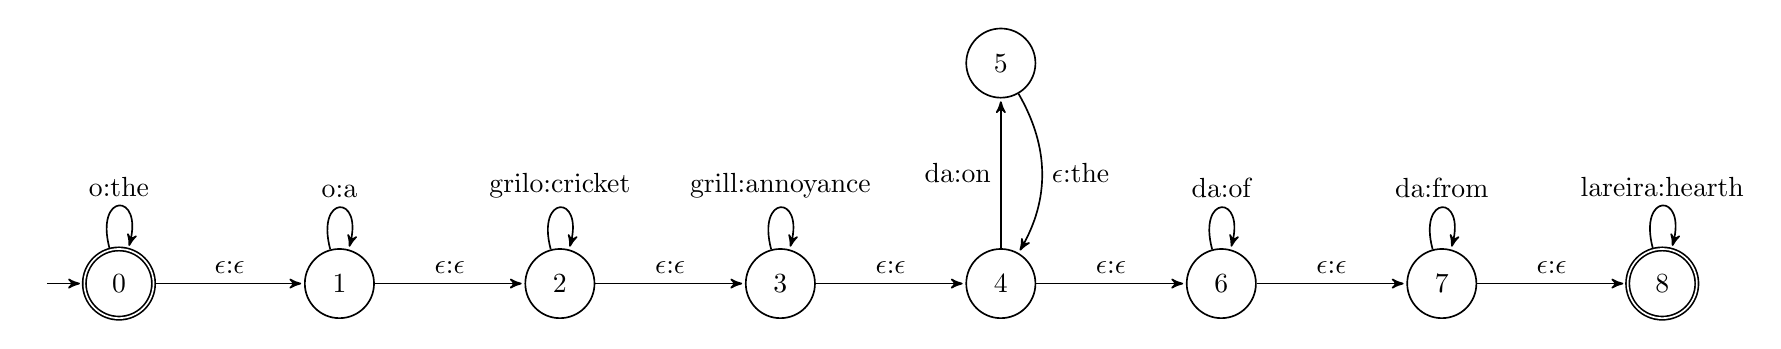
\begin{tikzpicture}[->,>=stealth',shorten >=1pt,auto,node distance=2.8cm,semithick]
  	\tikzstyle{every state}=[draw=black,text=black]
  	\node[initial,accepting,state,style={initial text=}] (A) {$0$};
  	\node[state] (B) [right of=A] {$1$};
	\node[state] (C) [right of=B] {$2$};
	\node[state] (D) [right of=C] {$3$};
	\node[state] (E) [right of=D] {$4$};
	\node[state] (F) [above of=E] {$5$};
	\node[state] (G) [right of=E] {$6$};
	\node[state] (H) [right of=G] {$7$};
	\node[state,accepting] (I) [right of=H] {$8$};
	
\path (A) edge [loop above] node {\ftext{o}:\etext{the}} (A);
\path (B) edge [loop above] node {\ftext{o}:\etext{a}} (B);
\path (C) edge [loop above] node {\ftext{grilo}:\etext{cricket}} (C);
\path (D) edge [loop above] node {\ftext{grill}:\etext{annoyance}} (D);
\path (E) edge node {\ftext{da}:\etext{on}} (F);
\path (F) edge [bend left] node {$\epsilon$:\etext{the}} (E);
\path (G) edge [loop above] node {\ftext{da}:\etext{of}} (G);
\path (H) edge [loop above] node {\ftext{da}:\etext{from}} (H);
\path (I) edge [loop above] node {\ftext{lareira}:\etext{hearth}} (I);

\path (A) edge node {$\epsilon$:$\epsilon$} (B);
\path (B) edge node {$\epsilon$:$\epsilon$} (C);
\path (C) edge node {$\epsilon$:$\epsilon$} (D);
\path (D) edge node {$\epsilon$:$\epsilon$} (E);
\path (E) edge node {$\epsilon$:$\epsilon$} (G);
\path (G) edge node {$\epsilon$:$\epsilon$} (H);
\path (H) edge node {$\epsilon$:$\epsilon$} (I);
\end{tikzpicture}
}
\end{textblock*}
}

	
}

\frame{
	\frametitle{Phrase permutations' translations with WL$d$}
\begin{columns}
\begin{column}{0.5\textwidth}
	
\newcommand{\biwldadjcond}{
\begin{array}{l }
\textcolor<2>{blue}{i = l}\\
\alert<3>{\oplus_k c_k = \bzero}
\end{array}
}

\newcommand{\biwldnonadjcond}{
\begin{array}{l }
\textcolor<5>{blue}{l < i \leq I} \\
\alert<6>{\delta(i', l) \leq d} \\
\oplus_k c_k = \bzero
\end{array}
}


\begin{math} %\small
 \left. 
  \begin{array}{l}
    \textsc{Item} ~~~~ {\itembrack{[1 .. I +1], \{0,1\}^{d-1}}} \\
    %\\
    \textsc{Goal} ~~~~ {\itembrack{I+1, C}} \\
    %\\  
    \textsc{Axiom} \\ 
	\drule{}{\itembrack{1, 0^{d-1}}}{} \\
    %\\  
    \textsc{Adjacent} \\ 
	\drule{\alert<1>{\itembrack{l, C}} \alert<2>{\angbrack{x_i^{i'} \ra y_j^{j'}}}}{\textcolor<4>{blue}{\itembrack{l + n, C' \ll n}}}{\biwldadjcond} \\ 
	~~ \text{where} \\
	~~~ \alert<4>{C' = \alpha_l^{i+1..i'}(C)} \\
	~~~ \text{$n = \#_1(C') + 1$} \\
%	~~ \alert<4>{\text{\small where $n = \#_1(C') + 1$}} \\
%	~~ \text{\small and $\#_1(C)$ is the number of leading ones in $C$} \\
    \textsc{Non-Adjacent} \\ 
	\drule{\itembrack{l, C} \alert<5>{\angbrack{x_i^{i'} \ra y_j^{j'}}}}{\itembrack{l, \alpha_l^{i..i'}(C)}}{\biwldnonadjcond} \\ 
	
  \end{array} 
\right.
\end{math}


\end{column}
\begin{column}{0.5\textwidth}
	\only<1>{\alert<1>{Permutation window}}
	\only<2>{\textcolor{blue}{Adjacent} \alert{phrase pair}}
	\only<3>{\alert<3>{No overlaps}}
	\only<4>{\alert<4>{update} and \textcolor{blue}{shift}}
	\only<5>{\textcolor{blue}{Non-adjacent} \alert{phrase pair}}
	\only<6>{\alert{distortion limit}}
	\only<7>{
	\begin{itemize}
		\item $O(Id^22^{d-1})$ states \\
		(phrases are limited in length)
		\item $O(tId^22^{d-1})$ transitions
	\end{itemize}
	}
\end{column}
\end{columns}


}

\frame{
	\frametitle{Generalising the rule set (ITG)}
	Simply extend the terminal rules
	\pause
	\begin{itemize}
		\item $X \ra X X$ \\
		direct order \pause
		\item $X \ra \angbrack{X X}$\\
		inverted order \pause
		\item $X \ra r_i$, where $r_i \in R$\\
		\textcolor{ForestGreen}{bilingual mappings}
	\end{itemize}
	\pause
	
	Examples \\
	
	\begin{tabular}{l}
	$X \ra \ftext{o}/\etext{the}$\\
	$X \ra \ftext{grilo}/\etext{cricket}$\\
	$X \ra \ftext{da}/\etext{on the}$\\
	\end{tabular}
	
	\pause
	
	The intersection mechanisms do the rest\\
	\begin{itemize}
		\item $O(I^3)$ nodes (phrases are limited in length)
		\item $O(tI^3)$ edges
	\end{itemize}

}

\frame{
	\frametitle{Recap 3}
	
	We have \pause
	\begin{enumerate}
		\item defined different models of translational equivalence
		\pause
		\begin{itemize}
			\item by translating words or phrases
			\pause
			\item in arbitrary order
			\pause
			\item or according to an ITG
		\end{itemize}
		\pause
		\item efficiently represented the set of translations supported by these models for a given input sentence \pause
		\begin{itemize}
			\item trivially expressed in terms of intersection/composition \pause
			\item a logic program can do the same \\
			(sometimes more convenient, e.g. WL$d$ constraints) 
		\end{itemize}
	\end{enumerate}
}


\frame{
	\frametitle{Remarks}
	
	Phrase-based SMT \precite{Koehn et al, 2003} \pause
	\begin{itemize}
		\item the space of solutions grows linearly with input length and exponentially with the distortion limit
	\end{itemize}
	\pause
	ITG \precite{Wu, 1997} \pause
	\begin{itemize}
		\item the space of solutions is cubic in length \pause
		\item however less efficiently packed, better motivated constraints on reordering
	\end{itemize}
	
}

\frame{
	\frametitle{Remarks (hiero)}	
	
	Hierarchical phrase-based models \precite{Chiang, 2005}
	\pause
	\begin{itemize}
		\item more general SCFG rules (typically up to 2 nonterminals)\\ \pause
		\item weakly equivalent to an ITG\\ 
		(same set of pairs of strings) \pause 
		\item purely lexicalised rules \\ 
		e.g. $X \ra \ftext{loja de antiguidades} / \etext{old curiosity shop}$ \pause
		\item as well as lexicalised recursive rules \\ 
		e.g. $X \ra X_1 \ftext{ de } X_2 \text{ / } X_2 \etext{ 's } X_1$ \pause
		\item no purely unlexicalised rules\footnote{Other than monotone translation with \emph{glue rules}} \\ \pause
		\item same cubic dependency on input length (as ITGs)
		%\item typically estimated heuristically from word-alignment\\
		%(lexical evidence helps here)
	\end{itemize}
	
}
	
	
	\section{Parameterisation}

\frame{
	\frametitle{What are we missing?}
	
	We have characterised the set of solutions ``backed'' by our transfer model\\ \pause
	\begin{itemize}
		\item these solutions are unweighted \pause
		\item there is no obvious way to discriminate between them \pause
		\item we cannot make decisions like that
	\end{itemize}
	
	\pause
	
	We are missing a parameterisation of the model
	\begin{itemize}
		\item the scoring function which will guide the decision making process
	\end{itemize}
}

\frame{
	\frametitle{Linear models}
	
	Let's call {\bf derivation}  \pause
	\begin{itemize}
		\item a translation string \pause
		\item along with any latent structure assumed by the transfer model \\
		e.g. phrase segmentation, alignment
	\end{itemize}
	\pause
	
	A linear parameterisation of the model is a function
	$$f(\mdd) = \sum_k \lambda_k H_k(\mdd)$$
	where \mdd is the derivation, and $H_k$ is one of $m$ feature functions\\
	
	~ \pause
	
	It assigns a real-valued score to each and every derivation \\
	
	~ \pause
	
	Think of it as a surrogate for translation quality at decoding time
}

\frame{
	\frametitle{Feature functions}
	
	Independently capture different aspects of the translation, such as
	\begin{itemize}
		\item adequacy
		\begin{itemize}
			\item translation probabilities
			\item confidence on lexical choices
		\end{itemize}
		\item fluency
		\begin{itemize}
			\item LM probabilities
			\item confidence on reodering
		\end{itemize}
	\end{itemize}
	
	
}

\frame{
	\frametitle{Independence assumptions}
	
	Our transfer model makes independence assumptions
	\begin{itemize}
		\item ``translation happens by concatenating isolated rules''
		e.g. flat mappings, hierarchical mappings
	\end{itemize}
	\pause
	
	~
	
	Certain aspects of translation quality comply with such assumptions\looseness=-1
	\begin{itemize}
		\item how likely a certain translation rule is \\
		e.g. relative frequency in a bilingual corpus
	\end{itemize}
	\pause
	
	~
	
	Certain aspects do not comply with such assumptions
	\begin{itemize}
		\item fluency as captured by an $n$-gram LM
	\end{itemize}
	
}

\frame{
	\frametitle{Structural independence}

\begin{textblock*}{110mm}(0.1\textwidth,0.30\textheight)

Suppose a set of derivations (e.g. monotone word mappings)\looseness=-1 \\

	
\scalebox{0.6}{

\begin{tikzpicture}[->,>=stealth',shorten >=1pt,auto,node distance=2.8cm,semithick]
  	\tikzstyle{every state}=[draw=black,text=black]

\node[initial,state,style={initial text=}] (A) {$0$};
\node[state] (B) [right of=A] {$1$};
\node[state] (C) [right of=B] {$2$};
\node[state] (D) [right of=C] {$3$};
\node[state] (E) [right of=D] {$4$};
\node[state,accepting] [right of=E] (F) {$5$};

\only<1>{\path[color=red] (A) edge node {\ftext{um}} (B);}
\only<1-2>{\path[color=red] (B) edge node {\ftext{conto}} (C);}
\only<1-3>{\path[color=red] (C) edge node {\ftext{de}} (D);}
\only<1-4>{\path[color=red] (D) edge node {\ftext{duas}} (E);}
\only<1-5>{\path[color=red] (E) edge node {\ftext{cidades}} (F);}
	
\only<2->{
	\path[color=blue] 
		(A) edge node {\etext{a}} (B)
			edge [bend right] node {\etext{some}} (B)
			edge [bend left] node {\etext{one}} (B);
}
\only<3->{
	\path[color=blue] 
		(B) edge node {\etext{narrative}} (C)
			edge [bend right] node {\etext{tale}} (C)
			edge [bend left] node {\etext{story}} (C)
			edge [bend right=60] node [below] {novella} (C);
}
\only<4->{
	\path[color=blue] 
		(C) edge node {\etext{of}} (D)
			edge [bend right] node {\etext{from}} (D)
			edge [bend left] node {\etext{'s}} (D);
}
\only<5->{
	\path[color=blue] 
		(D) edge [bend left] node {\etext{two}} (E)
			edge [bend right] node {\etext{couple}} (E);
}
\only<6->{
	\path[color=blue] 
		(E) edge node {\etext{cities}} (F)
			edge [bend right] node {\etext{towns}} (F)
			edge [bend left] node {\etext{villages}} (F);
}			
\end{tikzpicture} 

}

\only<7->{
When scoring complies with such ``structural independence''\\
}
\only<8->{\hfill \alert{we work with packed representations \\ \hfill(polynomial in input length)}}

\end{textblock*}
	
}


\frame{
	\frametitle{Structural independence: one extreme}

	If our features are fully compliant with structural independence \\
	~
	
\begin{center}
\begin{math}
\begin{array}{l r}
\only<2->{\mdd = \angbrack{e_1, \ldots, e_l} & \text{sequence of independent steps}\\}
\only<2-5>{& \\}
\only<3->{f(\mdd) = \sum_k \lambda_k H_k(\mdd) & \text{model factorises over features}\\}
\only<2-5>{& \\}
\only<4->{H_k(\mdd) = \sum_{e\in \mdd} h_k(e) & \text{features factorises over steps}\\}
\only<2-5>{& \\}
\only<5->{w(e) = \sum_k \lambda_k h_k(e) & \text{ergo, model factorises over steps}\\}
\end{array}
\end{math}
\end{center}

\only<6->{
\scalebox{0.6}{

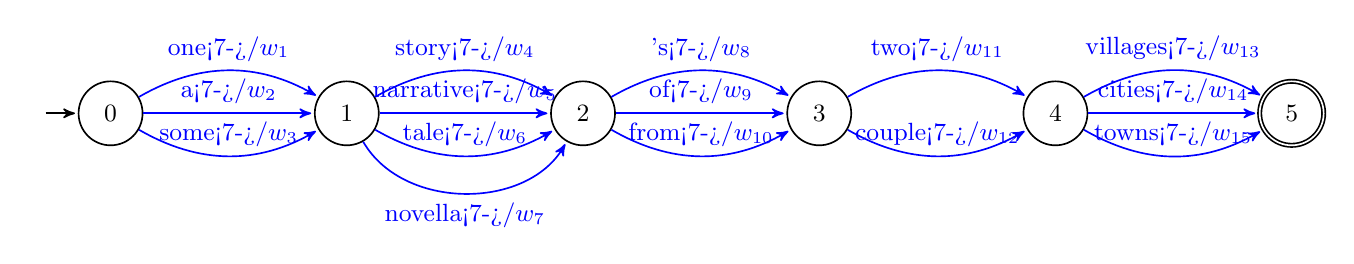
\begin{tikzpicture}[->,>=stealth',shorten >=1pt,auto,node distance=3cm,semithick]
  	\tikzstyle{every state}=[draw=black,text=black]
\small
\node[initial,state,style={initial text=}] (A) {$0$};
\node[state] (B) [right of=A] {$1$};
\node[state] (C) [right of=B] {$2$};
\node[state] (D) [right of=C] {$3$};
\node[state] (E) [right of=D] {$4$};
\node[state,accepting] [right of=E] (F) {$5$};

	\path[color=blue] 
		(A) edge node {\etext{a}\only<7->{/$w_2$}} (B)
			edge [bend right] node {\etext{some}\only<7->{/$w_3$}} (B)
			edge [bend left] node {\etext{one}\only<7->{/$w_1$}} (B);


	\path[color=blue] 
		(B) edge node {\etext{narrative}\only<7->{/$w_5$}} (C)
			edge [bend right] node {\etext{tale}\only<7->{/$w_6$}} (C)
			edge [bend left] node {\etext{story}\only<7->{/$w_4$}} (C)
			edge [bend right=60] node [below] {\etext{novella}\only<7->{/$w_7$}} (C);
	\path[color=blue] 
		(C) edge node {\etext{of}\only<7->{/$w_9$}} (D)
			edge [bend right] node {\etext{from}\only<7->{/$w_{10}$}} (D)
			edge [bend left] node {\etext{'s}\only<7->{/$w_8$}} (D);
	\path[color=blue] 
		(D) edge [bend left] node {\etext{two}\only<7->{/$w_{11}$}} (E)
			edge [bend right] node {\etext{couple}\only<7->{/$w_{12}$}} (E);
	\path[color=blue] 
		(E) edge node {\etext{cities}\only<7->{/$w_{14}$}} (F)
			edge [bend right] node {\etext{towns}\only<7->{/$w_{15}$}} (F)
			edge [bend left] node {\etext{villages}\only<7->{/$w_{13}$}} (F);
			
\end{tikzpicture} 
}}

\only<8->{
Efficiently packing $\Rightarrow$ efficient DP-based inference \\
\hfill \alert{(linear with the number of edges)}
}

}

\frame{
	\frametitle{Structural independence: the other extreme}

	Imagine a feature function that requires a complete translation
	\pause
	\begin{itemize}		
		\item unbounded LM \\
		e.g. via suffix arrays or distributed representations
		\item estimated overall translation quality (QE models?)
	\end{itemize}
	\pause
	Steps can no longer be weighted in isolation \pause
	\begin{itemize}
		\item it requires unpacking the representation \pause
		\item making dependencies explicit through the graphical structure
	\end{itemize}
	
	
}

\frame{

	\frametitle{An DP fails...}

\scalebox{0.6}{

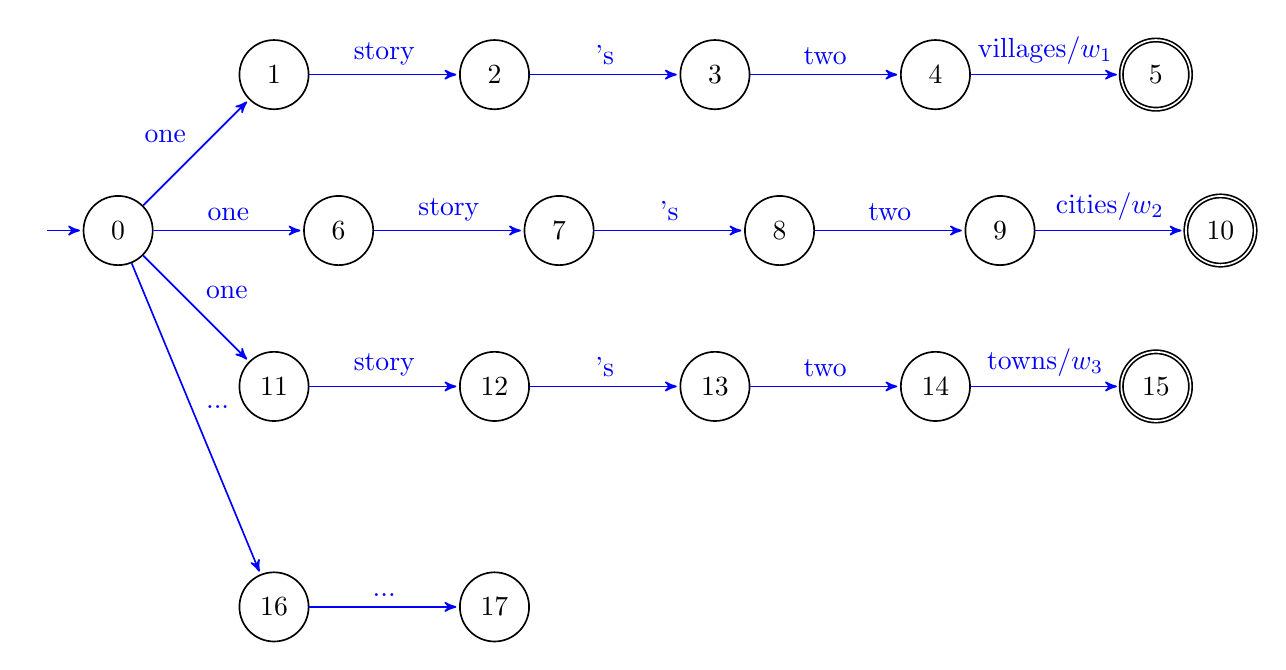
\begin{tikzpicture}[->,>=stealth',shorten >=1pt,auto,node distance=2.8cm,semithick]
  	\tikzstyle{every state}=[draw=black,text=black]
  	\tikzstyle{every path}=[draw=blue,text=blue]	

\node[initial,state,style={initial text=}] (q0) {$0$};
\node[state] (q1) [above right of=q0] {$1$};
\node[state] (q2) [right of=q1] {$2$};
\node[state] (q3) [right of=q2] {$3$};
\node[state] (q4) [right of=q3] {$4$};
\node[state,accepting] [right of=q4] (q5) {$5$};

\node[state] (q6) [right of=q0] {$6$};
\node[state] (q7) [right of=q6] {$7$};
\node[state] (q8) [right of=q7] {$8$};
\node[state] (q9) [right of=q8] {$9$};
\node[state,accepting] [right of=q9] (q10) {$10$};

\node[state] (q11) [below right of=q0] {$11$};
\node[state] (q12) [right of=q11] {$12$};
\node[state] (q13) [right of=q12] {$13$};
\node[state] (q14) [right of=q13] {$14$};
\node[state,accepting] [right of=q14] (q15) {$15$};

\node[state] (q16) [below of=q11] {$16$};
\node[state] (q17) [right of=q16] {$17$};

\path
(q0) edge node {\etext{one}} (q1)
(q1) edge node {\etext{story}} (q2)
(q2) edge node {\etext{'s}} (q3)
(q3) edge node {\etext{two}} (q4)
(q4) edge node {\etext{villages}/$w_1$} (q5);

\path
(q0) edge node {\etext{one}} (q6)
(q6) edge node {\etext{story}} (q7)
(q7) edge node {\etext{'s}} (q8)
(q8) edge node {\etext{two}} (q9)
(q9) edge node {\etext{cities}/$w_2$} (q10);

\path
(q0) edge node {\etext{one}} (q11)
(q11) edge node {\etext{story}} (q12)
(q12) edge node {\etext{'s}} (q13)
(q13) edge node {\etext{two}} (q14)
(q14) edge node {\etext{towns}/$w_3$} (q15);

\path
(q0) edge node {\etext{...}} (q16)
(q16) edge node {\etext{...}} (q17);
			
\end{tikzpicture} 
}

~

	Exhaustive enumeration 
	\begin{itemize}
		\item number of edges exponential with input length
		\item \alert{intractable}
	\end{itemize}

}

\frame{
	\frametitle{Not all is lost}
	
	Most features we can reliably estimate \pause
	\begin{itemize}
		\item are rarely sensitive to global context \pause
		\item are quite incremental \pause
		\item compromise between these extreme cases 
	\end{itemize}
	\pause
	
	$n$-gram LMs are good examples
	
	\begin{itemize}
		\item there are up to $|\Delta|^{n-1}$ contexts that must be made explicit \pause
		\item nodes must group derivations sharing the same context \pause
		\item polynomial, though often prohibitive

	\end{itemize}

}

\frame{
	\frametitle{Making context explicit (intuition)}

\scalebox{0.6}{

\begin{tikzpicture}[->,>=stealth',shorten >=1pt,auto,node distance=2.8cm,semithick]
  	\tikzstyle{every state}=[draw=black,text=black]
  	\tikzstyle{every path}=[draw=blue,text=blue]	

\node[initial,state,style={initial text=}] (q0) {$0$};
\only<2>{\node[state] (q1) [right of=q0] {$i$};}
\only<2>{\node[state] (q2) [right of=q1] {$ii$};}
\only<3->{
\node[state] (qOne) [above right of=q0] {$1$};
\node[state] (qA) [right of=q0] {$2$};
\node[state] (qSome) [below right of=q0] {$3$};
}
\only<4->{\node[state] (qTale) at (7,3) {$4$};}
%\node[state] (qTale) [above of=qNarra] {$4$};
%\node[state] (qNovel) [below of=qNarra] {$6$};
%\node[state] (qStory) [below of=qNovel] {$7$};

\only<5->{
\node[state] (qStory) at (12,-2) {$5$};
}

%\node[state,accepting] [right of=q4] (q5) {$5$};

\only<2>{
\path
(q0) edge node {\etext{a}} (q1)
	edge [bend right] node {\etext{some}} (q1)
	edge [bend left] node {\etext{one}} (q1);

\path
(q1) edge node {\etext{narrative}} (q2)
	edge [bend right] node {\etext{tale}} (q2)
	edge [bend left] node {\etext{story}} (q2)
	edge [bend right=60] node [below] {novella} (q2);	
	
}
\only<3->{
\path
(q0) edge node {\etext{a}/$w(\text{a})$} (qA)
	edge [bend right] node {\etext{some}/$w(\text{some})$} (qSome)
	edge [bend left] node {\etext{one}/$w(\text{one})$} (qOne);
}
\only<4->{
\path
(qOne) edge [bend left] node {\etext{tale}/$w(\text{one tale})$} (qTale)
(qA) edge node {\etext{tale}/$w(\text{a tale})$} (qTale)
(qSome) edge [bend right] node [below] {\etext{tale}/$w(\text{some tale})$} (qTale);
}

\only<5->{
\path
(qOne) edge [bend left] node {\etext{story}/$w(\text{one story})$} (qStory)
(qA) edge node {\etext{story}/$w(\text{a story})$} (qStory)
(qSome) edge [bend right] node [below] {\etext{story}/$w(\text{some story})$} (qStory);
}

			
\end{tikzpicture} 
}	
	
}

\frame{
	\frametitle{Recap 4}
	
	\begin{enumerate}
		\item a characterisation the space of solutions \pause
		\item a linear parameterisation of the model \pause
		\item impact of parameterisation on packed representations
	\end{enumerate}
	\pause
	
	What's left? \pause
	\begin{itemize}
		\item more examples of models and impact on representation
		\begin{itemize}
			\item distance-based reordering
			\item lexicalised models
			\item a global feature function
		\end{itemize}
		\item inference algorithms \pause
		\item techniques to make inference feasible for interesting models	
	\end{itemize}
}

	
	\section{Decision rules}

\frame{
	\frametitle{Picking one solution}
	
	What do we pick out of the (whole) weighted space of solutions? \\
	
	\begin{itemize}
		\item best translation
		\item ``minimum-loss'' translation
	\end{itemize}
}

\frame{
	\frametitle{Best translation}
	MAP \\
	
	$$\myy\ustar = \argmax_\myy \sum_{\opy[\mdd] = \myy} f(\mdd|\mxx)$$
	
	\pause 
	\begin{itemize}
		\item summing alternative derivations of the same string \\
		NP-complete: related to determinisation \citep{Simaan:1996:complexity} \\ 
	\end{itemize}
	
	\pause
	
	Viterbi (approximation to MAP)\\ 
	
	$$\mdd\ustar = \argmax_\mdd f(\mdd|\mxx)$$
	
	\begin{itemize}
		\item assumes the most likely derivation is enough
	\end{itemize}
}

\frame{
	\frametitle{Minimum Bayes Risk translation}
	
	MBR \\
	\begin{itemize}
		\item<2-> incorporates a loss (or gain) function 
	\end{itemize}
	
	\only<3>{
	$$\myy = \argmin_\myy \angbrack{\loss(\myy, \myy')}_{p(\myy'|\mxx)}$$}
	\only<4>{
	$$\myy = \argmax_\myy \angbrack{\gain(\myy, \myy')}_{p(\myy'|\mxx)}$$}
	\only<5-6>{
	$$\myy = \argmax_\myy \angbrack{\BLEU(\myy, \myy')}_{p(\myy'|\mxx)}$$}
	\only<7-8>{
	$$\myy = \argmax_\myy \sum_{\myy'} \BLEU(\myy, \myy') \alert<8>{p(\myy'|\mxx)}$$}
	\only<9>{
	$$\myy = \argmax_\myy \sum_{\alert<9>{\myy' \sim p(\myy'|\mxx)}} \BLEU(\myy, \myy')$$}
	\only<10->{
	$$\myy = \argmax_\myy \sum_{\myy'} \sum_{\alert<10>{\mdd' \sim p(\mdd'|\mxx)}} \BLEU(\myy, \opy[\mdd'])$$}
	
	\begin{itemize}
		\item<6-> assesses the risk associated with choosing any one translation
		\item<7-> requires the computation of expectations 
		\item<8-> which requires a \alert<8>{probability}
		$$p(\mdd|\mxx) = \frac{f(\mdd|\mxx)}{\sum_{\mdd'} f(\mdd'|\mxx)}$$
		\item<9-> can be estimated by \alert<9>{sampling translations}
		\item<10-> can be estimated from \alert<10>{samples of derivations}
		%\item<11-> \alert{have a look at project 14 ;)}\\
		
	\end{itemize}
}


\section{Decoding algorithms}

\frame{
	\frametitle{DP-based Viterbi}
	
	Explore a truncated version of the full space \pause
	\begin{itemize}
		\item only a budgeted set of outgoing edges form each node \\ \pause
		\begin{itemize}
			\item beam search: exhaustively enumerates outgoing edges, ranks them, prunes all but $k$-best \pause
			\item cube pruning: enumerates $k$ edges in near best-first order \pause
%			\item incremental search: enumerates the $k$-best edges \pause
		\end{itemize}
	\end{itemize}
	
	In order to compare hypotheses more fairly \pause
	\begin{itemize}
		\item future cost estimates \pause
		\item heuristic view of outside weights \pause
		\item cheap dynamic program that estimates the best possible way to complete any translation prefix \pause
	\end{itemize}
	
	\hfill \citep{Koehn+2003:pbsmt} \\
	\hfill \citep{Chiang:2007}
}

\frame{
	\frametitle{DP-based MBR}
	
	Uses derivations in an $n$-best list as samples \pause
	\begin{itemize}
		\item arguably poor proxy to samples \pause
		\item arbitrarily biased (due to pruning) \pause
		\item centred around the Viterbi solution by design (due to beam search)
	\end{itemize}
	\pause
	\hfill \citep{Kumar+2004:MBR}\\
	\hfill \citep{Tromble+2008:LMBR}

}

\frame{
	\frametitle{Sampling}
	
	Gibbs sampling \pause
	\begin{enumerate}
		\item start with a draft translation \pause
		\item resample from posterior (not all simultaneously): \\ segmentation, phrase order, phrase selection \pause
		\item repeat 2 
	\end{enumerate}

	\pause
	Adaptive rejection sampling \pause
	\begin{enumerate}
		\item design a simpler upperbound (e.g. unigram LM) \pause
		\item sample from it \pause
		\item assess or reject at the complex distribution (e.g. $5$-gram LM) \pause
		\item rejected samples motivate refinements of the upperbound \pause
		\item repeat 2-3 until acceptance rate is reasonable (e.g. 5-10\%) 
	\end{enumerate}
	
}

\frame{
	\frametitle{Sampling}

	Disadvantages \pause
	\begin{itemize}
		\item hard to do it without introducing bias \pause
		\item might require large number of samples
	\end{itemize}
	\pause
	
	Advantages \pause
	\begin{enumerate}
		\item broad view of distribution \pause
		\item potential to incorporate arbitrarily complex features \\ 
		(at the sentence level at least) \pause
		\item sometimes unbiased \pause
		\item ideal for MBR and tuning \pause
		\item typically stupid simple to parallelise
	\end{enumerate}
	

}	

    \frame{
        \frametitle{Thanks!}
        
        Questions?

    }

	% Trick to discount the title page and the table of contents from the total number of frames
	% and to discount any backup slides which should be place after these instructions
	% All your regular slides come before this point	
	\appendix
	\newcounter{finalframe}
	\setcounter{finalframe}{\value{framenumber}}

	%\input{background}
	%
\frame[plain]{
	\frametitle{Earley intersection}
	
	\begin{footnotesize}
	\begin{align*}
	\textsc{Axioms} & \\
	& \drule{}{\itembrack{S' \ra \bullet S, q, q}}{q \in I} \\
	\textsc{Goal} & \\
	& \itembrack{S' \ra S \bullet, q, r} ~ q \in I \wedge r \in F\\
	\textsc{Scan} & \\
	& \drule{\itembrack{X \ra \alpha \bullet x \beta, q, s}}{\itembrack{X \ra \alpha x \bullet \beta}}{\angbrack{s, x, r} \in E}\\
	\textsc{Predict} & \\
	& \drule{\itembrack{X \ra \alpha \bullet Y \beta, q, r}}{\itembrack{Y \ra \bullet \gamma, r, r}}{Y \ra \gamma \in R} \\
	\textsc{Complete} & \\
	& \drule{\itembrack{X \ra \alpha \bullet Y \beta, q, s}\itembrack{Y \ra \gamma \bullet, s, r}}{\itembrack{X \ra \alpha Y_{s,r} \bullet \beta, q, r}}{X \neq S'} \\
	\textsc{Accept} & \\
	& \drule{\itembrack{S' \ra \bullet S, q, q}\itembrack{S \ra \gamma \bullet, q, r}}{\itembrack{S' \ra  S_{q,r} \bullet, q, r}}{r \in F} 
	\end{align*}
	\end{footnotesize}

	
}



	\frame[allowframebreaks]{ \frametitle{References}
        \bibliographystyle{plainnat}
        \bibliography{waziz}
	}			

	
	
	% Trick to discount regular frames from the total of backup frames
	\setcounter{framenumber}{\value{finalframe}}
	
	
\end{document}

%\xrightarrow[below]{above}
%\overset{x}{\rightarrow}
%\underset{x}{\rightarrow} 